\chapter{Origin and Dispersal of Iron in India}\label{chapter3}

\lhead[\small\thepage\quad chapter III]{}

The period around the closing centuries of the $2^{\rm nd}$ millennium BCE witnessed a changing configurations due to the emergence and adaptation of newer technologies. The technologies provided incentive and the infrastructure for material prosperity and overall growth. The innovative changes set the pace for a relatively vigorous socio-economic and techno-cultural change. One of the important technological innovations that took place during the period spanning over the $2^{\rm nd}$-$1^{\rm st}$ millennium BCE was the advent and development of iron metallurgy in the Indian subcontinent. In the large and diverse eco-zones of Indian subcontinent, iron technology made appearance in divergent contexts and in different ways. The exact time and circumstances of the introduction and adaptation of iron has been investigated at different levels. In regions closer to the raw material experiments could have started easily if need for metal was felt. In other areas, the circumstances differed. Therefore, a different approach to understanding of advent and adaptation of emerging technologies has to be adopted. It is desirable to address the issue of beginning of iron in India in different eco-zones which were not easily accessible due to geographical barriers. We will attempt to do so in course of discussions that ensue. Each zone may present us with divergent chronological framework and adaptation pattern. New evidences are being brought forth by excavations being carried out every year. Radiometric characterizations from excavated sites are pushing back the antiquity of iron in India. In view of fresh light being thrown by issue of iron technology, the related issues have to be addressed afresh while taking cognizance of the earlier viewpoints expressed by historians/ archaeo-metallurgists from time to time. Broadly speaking, there are two main viewpoints on origin of iron in the Indian subcontinent, that is, 1- diffusion of iron from outside; 2- indigenous origin of iron. We propose to examine both the viewpoints in some detail here.  First we take a look at the diffusionistic theory of advent of iron in India. Three basic points were raised in this regard:


(1) Metallurgists strongly believed that iron technology is too complex to be learnt independently (Forbes 1950). It had to be learnt and perfected under the guidance of artisans who were well adept in the process of iron working\endnote{This view is no longer tenable in view of recent researches suggesting accidental discovery of iron as a by product of copper smelting.}.

%~ (1) Metallurgists strongly believed that iron technology is too complex to be learnt independently (Forbes 1950). It had to be learnt and perfected under the guidance of artisans who were well adept in the process of iron working.

 
(2) It was strongly believed that Aryans had entered India with horses and superior weapons (iron?) overpowered the indigenous inhabitants and occupied the land of seven rivers \textit{(saptasaindhav desh)}. There is reference to \textit{ayas} in the Rigveda, the earliest Aryan treatise. 
 
 (3) Iron was introduced by the Greeks or Bactrians as they were present in north-west India. This view was proposed on discovery of iron from sites like Taxila in the early parts of the $20^{\rm th}$ century the British archaeologists who were at the helm of affairs at the time. Since the Bactrians and Greeks had ruled the North-western part of the subcontinent during $5^{\rm th}$-$4^{\rm th}$ centuries BCE and iron was found in those strata, it reinforced the assumption that iron was brought in by them (Gordon 1958: 50-78). Similarly, Sir Mortimer Wheeler (1958) recovered iron artifacts from excavations of megalithic sites like Brahmagiri, Maski etc. Interestingly, as per the norm and the colonial temper, both the archaeologists had ruled out the possibility of use of iron in the subcontinent prior to 600-500 BCE. These views have to be examined closely in light of recent researches. 
 
The other set of scholars worked on literary evidences on iron. Scholars like Neogi (1914) and M.N. Banerji (1929) who had gone into the rich literary accounts of India chose to closely examine the occurrence of ayas which meant iron in Sanskrit. Reference to \textit{ayas} in Early texts, including the Rigveda led to assumption that antiquity of iron coincides with early Vedic period. It has been argued that the Rigvedic Aryans were well conversant with iron \textit{(ayas)} technology wherein one comes across tools and implements made with \textit{ayas}. The question is what did Vedic \textit{ayas} stand for? The term \textit{ayas}, it seems had different connotations. More in-depth researches show that the term \textit{ayas} is a generic term used for metal. As we will see below, intense debate followed on the etymology of word ayas and whether it stood for iron in the Early Vedic texts.


Lallanji Gopal (1961) synthesized the existing literary data and came to the conclusion that the word \textit{ayas} in the \textit{Rigveda}, stood for metal in general, not specifically for iron.~According to him iron was introduced in India during the Later Vedic times. This interpretation of the word \textit{ayas} at the earliest stage is significant indeed to the issue of introduction of iron in India. A detailed analysis of the prevalent views on the advent of iron in India is called for here. In recent years (as discussed in chapter II), scholars have taken a second look at the diffusionistic viewpoint of introduction of iron due to the fact that iron was more probably a by-product of copper or lead metallurgy. However, we would first take up the theories of diffusion of iron technology followed by the alternative viewpoints. 

The theory of diffusion took roots because it was believed by a set of scholars, especially Indologists that the Aryans migrated from a common homeland. It was further argued that the Aryans dispersed and settled in different parts of the world in course of their move; this included the Indian subcontinent. This has given rise to theory of diffusion of people and/or ideas. This includes advent of iron technology in India. It is another matter, however that the idea of Rigvedic Aryans being outsiders has now been contested by scholars on the basis of researches being carried out in the field of genetics, especially DNA of population from the concerned regions. However, following the earlier theories propagated regarding the Aryan immigration, we would first take a look at the diffusionistic viewpoint of origin of iron in India.	

\vspace{-.5cm}

\section*{The Theory of Diffusion of Technology}\label{chapter3-section-1}

\vspace{-.2cm}

The philological evidence suggesting similarities between Indo-European languages and Sanskrit, the common features noticeable in the Iranian sacred text the \textit{Avesta} and the \textit{Rigveda}, the oldest Ayran text and the inscriptional evidence like the Boghaz Keui (dated 1365 BCE, a treaty between Hittite king Shubbiluliuma and the Mitanni King Mattiuaza, referring to four Vedic gods) have given rise to a theory of common homeland of authors of these cultures. The linguistic affinity had gained cultural attributes in due course of time. In the specific context of introduction of iron technology in India, the theory of Aryan immigration from the west, though debated has come in handy. It is believed that iron, which was known to the people of Asia Minor in the $2^{\rm nd}$ millennium BCE, entered the Indian sub-continent with the immigrating Aryans. As examined in detail above (also see Tripathi 2001: 57-78), there are indisputable literary references to the knowledge and use of iron in the pre-1200 BCE period in Mitanni, Hittite and Egyptian records. The king of Mitanni, Tushratta sent the Egyptian Pharaoh, a dagger with iron blade with lapis lazuli studded gold handle (using 14 ‘shekels’ of gold) (quoted by Maddin 1982: 16).

Another reference belonging to the early $13^{\rm th}$ century BCE narrates the contents of a letter of a Hittite king Hattusilius III to the king of Assyria, mentioned above, “As for the good iron about which you wrote to me, there is no good iron in my store house in Kizzuwatna. The iron (ore?) is (of) too low (a grade) for smelting. I have given orders and they are (now) smelting good iron (ores?). But up till now they have not finished, I shall send (it) to you. Meanwhile I am sending to you a blade of iron for a dagger.”(Maddin op cit, 16-17). These passages are sufficient to prove that iron was a precious, prized and naturally also a scarce commodity at this stage. The metal however was being smelted in small amounts sporadically in some parts of the ancient world. The Hittites kept the knowledge of iron working a closely guarded secret, confining the art to the Anatolian Plateau till about 1200 BCE. Their monopoly was broken by disruption of the Hittite Empire by the Thraco-Phrygian invaders who forced the former to migrate to the peripheries of the Assyrian Empire. Around this very time the use of iron objects multiplies and the world witnessed large-scale migrations by warrior tribes with superior weapons, horses and horse-drawn chariots.

In close succession to this incident (c.~1000 BCE), Ghirshman\break (1954~:~73) observed two perceptible phenomena in the Iranian plateau: The invasion of the Indo-Europeans and the increased use of iron in Iran. In this region, iron was first noticed in the necropolis of Sialk, Cemetery-A along with a new grey ceramic. Iron, however was restricted to just a few pieces as part of royal costume being exclusively ornamental in nature. It assumed a utilitarian role only in the succeeding phase in Cemetery-B. The number of objects increased considerably from a couple of objects in previous period to a noticeably large number as well as a diversified typology reflected in a variety of objects like swords, daggers, shields, javelins, arrowheads, horse bits, head and chest ornaments of horses along with utensils and ornaments like anklets. This has been interpreted as an incursion of new cultural elements in Iran introduced from farther west or north.

In western Iran, Young (1976) defined a three-fold stratification of emergence of iron, calling them Iron I, Iron II and Iron III. Iron makes its earliest appearance by way of stray occurrences primarily as bi-metallic objects in the pre-1000 BCE period, classified as Iron I. Its presence is restricted to its use by a selected few of the society. A grey pottery is associated with this cultural phase impinging on the local Bronze Age cultures. Young held that there were widespread migrations in the western part of the Iranian Plateau in this period. There were new pottery traditions and also change in the pattern of use of metals. Iron was introduced here at this stage by itinerant metal smiths or through some kind of trade. Young cites the parallel of a known situation of influx of gypsies in certain parts of the world.

Interestingly, there is a gap between Iron I and Iron II according to Young. Iron I has been dated between \textit{c}. 1300/1250-1100 BCE. Iron II, according to Young is datable roughly to about 1000-800 BCE. Geographically, India is close to the Iranian borders. It is likely, that there were intermittent folk movements into India through this region. The inherent similarity between Avesta and Rigveda corroborates familiarity  between the two neighbouring people.~ This has given rise to the assumption that iron was brought in India by these incoming tribes (the Aryans?) through Iran. (It is noteworthy that there is a near absence of iron in Iron I level dated between 1300-1100; it means that they were not the people who could introduce iron in India). Recently, D.~P.~Agrawal (1998, 2002) has underlined the – linguistic as well as geographical and migratory pattern of movement of people into the Central Himalayas. Agrawal has related this to the beginning of iron in this part. The presence of cist burials with use of iron in Kumaon region is significant in this respect. The presence of the Caucasoid racial elements in the population of Central Himalayan region is said to be a noteworthy feature in this regard. 

Similar evidence of burials of skeletal remains with Caucasoid features has also been brought to light in China recently. The richness of iron ore and presence of iron working tribes from time immemorial give credence to the hypothesis of diffusion of people in this region. Iron has been shown to be present in about 1000-800 BCE in Kumaon – Garhwal region.~There exists a possibility of migrations and technology transfer through the immigrating folk at least in these Himalayan zones (Agrawal and Tripathi 1995, Agrawal and Kharakwal 1998). Future research may throw more light on it. With this, we may go back to the issue of iron in \textit{Rigveda}. To evaluate the hypothesis of introduction of iron in India with incoming Aryans through the Iranian plateau, we need to examine in depth- a) the evidence of iron in \textit{Rigveda}; b) the cultural material including iron objects in Indo-Iranian borders for similarities that followed to substantiate the said intrusions by the Aryans in the region.

\vspace{-.4cm}

\subsection*{1. I. Iron in \textit{Rigveda}}\label{chapter3-subsection-1}

\vspace{-.2cm}

The composers of \textit{Rigveda} call themselves Arya-the noble one, a fine or superior people. It is well known and needs no elaborations here that there was some kinship bond between them and the people of the \textit{Avesta} and that the two separated at some point of time. There is no definite evidence to suggest that the Aryans who lived in India in the \textit{‘sapta saindhav desha’} (the land of seven rivers) came from outside nor they had prior knowledge of iron technology and that they brought iron weapons with them. We do come across the word \textit{‘ayas’} which stands for iron in later Vedic times. But we are faced with several problems here, such as: what was the original connotation of the word \textit{‘ayas’}? Did the Rgvedic \textit{‘ayas’} stand for iron? It is relevant for the present discussion. Scholars have examined it time and again and various interpretations are available to us today. M.~N.~Banerji (1927, 1929, 1932), N.~R.~Banerjee (1965), Gopal (1961), Roy (1984), Tripathi (1994, 1997) etc. have taken a close look and have offered interpretations of the word \textit{ayas}. M.~N.~Banerji, N.~R.~Banerjee and S.~N.~Roy have come to the conclusion that the Rgvedic \textit{‘ayas’} stands for iron; consequent to this they conclude that iron in India is an outcome of India’s relations with the Aryan tribes coming in India from the west. On the other hand, Gopal and the present author argue that in the initial stage the term \textit{‘ayas’} stood for metal in general. The author also feels that adjectives \textit{Krishna}  or \textit{Shyama} and \textit{Lohita} were prefixed to \textit{ayas} at a relatively later stage in \textit{Yajurveda samhita} with the beginning of iron to distinguish the `black metal` (\textit{Krishna ayas} or \textit{Shyama ayas} = iron) from the red metal (\textit{‘Lohita ayas'} = copper). As stated above, it is more likely that the word \textit{‘ayas’} was a generic term for metal interchangeably used to denote iron or copper till much later date as is clear from literary sources. If so, one wonders whether the Early Aryans, even if they came from outside had knowledge of iron.

A quick look at the precise context of occurrence of the word \textit{ayas} in Rigveda may be useful here. There are ten such references in Rigveda. In the verse I.CLXIII.9 there is a description of horse of god Indra whose colour is like \textit{ayas}, which shines, in sharp contrast to the golden rays of the sun. In Rg. X 99.8 the word is used in the sense of physical strength \textit{ayopasti} – strong powerful hands like one made of sharp \textit{‘ayas’}. The other two references are to (X 79.6) \textit{asi} or axe with sharp cutting edge and (I, 162, 20) a sword or dagger having an excellent edge. Rigveda X 112.2 and X 72.2 refer to the artisan \textit{(Karmar)} working with \textit{‘ayas’} using bellows. M.N. Banerjee thinks that it is only the ironworker who uses bellows and therefore these verses specifically refer to ironworkers. Rigveda VI 3.4 describes molten metal (\textit{‘dravi’}-liquified). The next reference X 31.3 uses the word \textit{‘damdhamant’} or \textit{‘samdamanti’} interpreted as ‘inspiring’ or ‘leading to’ by Sayana, the commentator. Griffith translates it in the sense of welding. M.~N.~Banerjee thinks that it indicates joining two pieces of metal after heating them.

If we take a close look at these contexts most of them appear to be more suitable for copper than iron. The earliest reference is only indicative of the colour. It may be interpreted both ways – red or black. Similarly, hands or sharp nails could be strong like copper-bronze or iron both. We have come across axes or razor blades of copper-bronze in early cultures right from early Harappan and Chalcolithic cultures. On the other hand, swords or daggers of iron appear much later though axes have been found.

It is not correct to assume that metallic iron, especially the wrought iron of the earliest phases, was stronger and better suited for weapons and other sharp edged tools. We have noted before (chapter II) that good bronze,

which has undergone through the process of annealing, has the strength of 1,20,000 P.S.I. (per square inch) while a wrought iron (with no carbon) has the strength of only 40,000 P.S.I. We know that the early iron found in India was wrought iron having no carbon in it. Thus technologically also the strong, sharp weapons of Rigvedic people were more likely to be that of copper–bronze than of iron, as indicated in similes and metaphors in the literature. This gets further corroboration a reference in the Rigveda (VI 3.4), which clearly narrates about to liquefaction of metal ayas. We know for definite that it was copper or bronze, which was liquefied. It reached a molten state at the time of smelting as well as casting of objects. Iron, on the other hand was produced in semi-solid state in the form of a bloom which had to be hammered and treated repeatedly to extricate the trapped residue in the form of slag and consolidate the iron into a homogenised metallic ingot. Interestingly, all the above references except for two are from the late sections of Rigveda. Thus technologically speaking, the passages making a mention of \textit{‘ayas’} are more likely to be suggesting copper-bronze than iron. If iron was not known to the Rigvedic Aryans, it would be difficult to sustain the argument that the knowledge of iron was acquired from outside from the brethren who occupied the distant lands outside the \textit{‘sapta sandhava desha’}. It will be in fitness of things to look for evidence of iron on the borders of India to see if chronologically there is a case for early occurrence of iron so as to influence transfer of technology to India through that route. 

\vspace{-.3cm}

\subsection*{1.II. Archaeological Evidence of Iron on the\\ Borderlands}\label{chapter3-subsection-2}

\vspace{-.2cm}

Archaeologically, the area adjacent to Iranian borderlands, modern Baluchistan (extending over Indo-Iranian plateau) has yielded a large number of cairn burials. Stein (1929) has reported as many as 5100 cairns. Many of these cairns have yielded iron objects along with copper-bronze objects and other cultural material along with pottery. Gordon (1950) suggested Iranian connections of Sialk Cementery B and the cairn burials of Baluchistan on the basis of similarities in pottery, burials and the metal objects. However, Lamberg-Karlovsky and Humphries (1968) disapprove of the ‘Sialk B connections’ or Indo-European movements to east’ towards the cairn burials of Baluchistan because of lack of ‘convincing parallels’. The ecology also plays a role in isolating this area as the “natural barriers of mountain desert in Baluchistan and southeast Iran have isolated the inhabitants from the domination of any neighbouring power in the $20^{\rm th}$ century AD. Thus, it seems likely that the occupants of Baluchistan, separated from both east and west, always maintained a relatively independent existence” (Lamberg-Karlovsky and Humphries, 1968). The distinctive painted pottery types could not readily be related to the Iranian Plateau or to the painted pottery tradition further to the east. Talking of the possible areas exerting their influence on the Dashtiari and interior Baluchistan, one must look-first to the Persian Gulf trading areas as an outside source of contact. Secondly, there is a connection among the cultures of the northwest India area. The Iranian plateau is an un-distinguished third”.

A close comparison of chronology, typology and pottery traditions of Baluchi cairns and that of North India tends to lend weight to the contention of Lamberg Karlovsky and Humphries (quoted above). The burden of archaeological evidence does not favour the thesis of diffusion of iron into India from the neighbouring West Asian and Central Asian countries. Firstly, a closer examination of tool typology in Iranian and Afghan sites and those in Sindh and Baluchistan area display little common features with iron objects of mainland India. Secondly, the cultural material corroborates the typological study, \textit{i.e.} the two areas appear to be culturally distinct. Thirdly, the chronological considerations go against any notion of diffusion. On Iran-Afghan sites as well as Indian North-west, iron emerges more or less simultaneously \textit{viz}. around 1100-1000 BCE. In recent years, the Swat-Gandhar region has yielded ${\rm C}^{\rm 14}$ dates going back to circa 1200 BCE. It may, however be noted that recent $^{14}{\rm C}$ dates from the middle Ganga Plain sites are much earlier than this.

\vspace{-.3cm}

\subsection*{1. III. Iron in China}\label{chapter3-subsection-3}

\vspace{-.2cm}

Having examined the circumstances and processes of the advent of iron in the neighbouring countries on the western sides of India, it may be proper now to look in the opposite direction. On the eastern and north-eastern neighbourhood of India is situated China. There is a large mountainous zone of the Himalayas connecting the two countries. There is definite evidence of the existence of interaction between India and China, right from the Neolithic times. There are clear indications of cultural exchange in the sites like Burzahom and Gufkral in the Kashmir Neolithic culture. Presence of jade beads, ring stones and axes with holes at both ends, burial of a dog are some definite proofs substantiating the contacts between these two regions. At the site of Gufkral iron appears for the first time in the post-Neolithic, megalithic phase. The earliest iron there comes from the burials dated by the TL dates to 1800-1700 BCE. In the very next phase (without any break) iron shows up in the megalithic burial culture at Gufkral that has been dated by the excavator to 1400 BCE. Recently $^{14}{\rm C}$ dates take back the antiquity of iron bearing levels to 1900 BCE (uncelebrated date). Such early date of iron bearing deposit is significant indeed. It may be worth examining the evidence of the earliest occurrence of iron in China with a view to examine the genesis of iron technology in this region.

China has a unique position in the Old World civilizations, being the only place where cast iron comes to be used at an early age. Cast iron was hardly used in Mesopotamia, Anatolia, in the Aegean or central Europe; it is apparently an invention of the ancient Chinese metal craftsmen. Though metallurgists like Cyril Stanley Smith do not quite support the contention of independent origin of metallurgy including that of China,``this by no means denies that there is something uniquely Chinese in the technique and the beauty of the superb bronzes of Shang and Chou China, but this seems to lie in the making of moulds and the decoration on them, not necessarily in the origins of metallurgy itself" (Smith 1973: 23).

One agrees with Smith that the Chinese metalworkers were ingenious in moulding beautiful bronze artifacts; there is every chance that using the same ingenuity they could master iron casting. As opposed to Smith's contention, Renfrew (1986:~145) has argued, “It has effectively been demonstrated that metallurgy in the new world had separate origins and developments from those in the Old World. It is even likely that metallurgy in China developed independently from that in West Asia. It has been argued on several occasions that there is a good case for the independent origin of metallurgy in South-East Europe. The same is true of Iberia". Thus origin of metallurgy is no longer taken to be an outcome of diffusion of people or ideas as was earlier believed to be. This is true in the case of China, as argued by Tylecote (1992: 75),

{\footnotesize “… China was to be the one country where iron technology was to take, a different course; towards cast iron rather than wrought iron, and it is therefore possible that ferrous metallurgy evolved independently from the highly sophisticated non-ferrous techniques of the region. The same sort of accident that produced recognizable ductile iron at the bottom of a copper smelting furnace could, under certain conditions, have produced cast iron and the Chinese would have realized that they had found a bronze substitute". }

\newpage

This view of Tylecote has been corroborated by the tool typology even at the early levels of occurrence of iron in China. Jueming also supported Tylecote saying that iron in China is an outcome of bronze metallurgy around 700-600 BCE. At the earliest stage balls were found at Liuhe and cauldron at Changsha in around 600 BCE. Iron soon replaced copper-bronze and even stone. A rich variety of commodities like ploughshare, spade, sickle, axe, adze, chisels, arrows, cloth-hooks etc. were discovered. Even moulds used in manufacture of iron objects were found at sites like Xinlung. The technology developed in due course of time for producing excellent quality malleable iron. To quote Hua Jueming, 

{\footnotesize “..we can conclude without any exaggeration that without the wide application of the toughening, it would have been impossible for cast iron to be so widely used during the Warring States. It was precisely this wonderful invention that played a historical role in the advancing of early Chinese Iron Age. This technique was perfected during the Han dynasty at the foundry at Tienshangou, Gongxian. On analysis the structure represents typical spherical graphite. (It may be noted that this technology was invented in Europe by J. H. Morrogh, as late as 1947)".}

For the discovery of cast iron in China Jueming credits the highly developed bronze industry with efficient furnace design (Muozi advises, ``each stone should be equipped with four bellows"), mechanical ventilators and selection of good refractory material. The incidence of cast iron could be possible in the furnaces generating high temperature due to strong draughts. Grey iron was obtained in the western Han and also in a foundry at Zhengzhou in eastern Han. These furnaces were 5 to 6 meters high having 50 cubic meter capacities. In certain areas blast systems were driven by water – the `Shuipai' or hydraulic expeller.

{\footnotesize ``Thus, cast iron is the foundation of Chinese iron metallurgy. Its early invention and wide application created a specific style of its own with the invention of puddling iron in western Han and soon afterwards the uniquely Chinese guan steel, China firmly established its specific iron and steel system".}

The 50 tonne lion statue is the product of this technique – a manifestation of an extraordinary skill! Even if there was an early occurrence of iron in China, it did not pass the know-how to India as the two regions had quite distinct metallurgical traits.

\newpage

This brief discussion of the advent of Chinese iron in antiquity makes it clear that (1) Chinese iron was in all probability an independent invention of the bronze and copper smiths; (2) though both wrought iron and cast iron were in use at the early levels, it is the latter which gained popularity in China; (3) they were the only ancient civilization of the world to cast colossal statues like a 50 ton lion figure; (4) and last but not least, both in time and technique, there is little similarity in the iron production between India and China; (5) Iron had a longer antiquity in India going back to 1800-1700 BCE while it started in the opening centuries of the first millennium BCE in China. India never adopted the cast iron technique of iron making. Therefore, it is not likely that introduction of iron in India was in any way influenced by China or its neighbourhood. On the contrary, there exists a strong case of diffusion of knowhow from India to China. 

The following points that emerge from the foregoing discussion are significant:
\begin{itemize}
\item[1.]In the Iranian plateau at the earliest stage iron was very scarce and was confined to graves only. Importantly enough, there was also a gap between this stage and the next stage. An uninterrupted use of iron starts only around 1100-1000 BCE.

\item[2.] In the neighbouring regions of the Indian borders, none of the areas appear to be in a position to pass on knowledge of iron metallurgy to India. Chronologically or typologically these regions are distinct and disparate.

\item[3.] The Rigvedic society does not seem to possess iron technology therefore their interaction with Avestan or other brethren is ruled out as source of iron technology.

\item[4.] It is well established now that iron metallurgy was a by-product of copper or lead working. The concept that iron metallurgy being too complex had to be learnt from the people adept in it, no longer holds ground.

\item[5.] If iron did not reach India through the western source, we may now explore the possibility of an indigenous origin of iron in India. As $^{14}{\rm C}$ dates from recent excavations push back the antiquity of iron in India, we need to take a fresh look at the alternative viewpoint of beginning of iron in India.
\end{itemize}

\vspace{-.5cm}

\section*{Indigenous Origin of Iron in India}\label{chapter3-section-2}

\vspace{-.2cm}

In recent years interesting evidence of early use of iron warrants fresh thinking on the antiquity of iron in India. The balance seems to tilt in favour of an older and indigenous origin of iron. It is therefore necessary to examine afresh the evidence available to us from the latest archeological researches going on in India. The maps (Fig.~\ref{chapter1-fig001},~\ref{chapter1-fig002} and ~\ref{chapter1-fig004}) show the important Iron Age cultures and different cultural zones in which early iron sites have been discovered. In addition to the archaeological sites, number of ethnological evidences have been brought to light from time to time (Fig.~\ref{chapter1-fig003}). 

\vspace{-.48cm}

\subsection*{2.I. Iron in the Chalcolithic Milieu}\label{chapter3-subsection-4}

\vspace{-.2cm}

In majority of cases iron in India makes its earliest appearance in a Chalcolithic setting. However, the incidence of iron at Ahar, (district Udaipur, Rajasthan) a Chalcolithic site, almost revolutionized the theories of advent of iron in India in early seventies. M.~D.~N.~Sahi (1979) pointed out the anomalies in the report of Ahar (Sankalia \textit{et al}. 1969). According to the original report of Ahar iron was said to have started with NBP (Period II) around 600-300 BCE in this part of Rajasthan. Period I having three subdivisions – Ia, Ib and Ic, belonged to the Chalcolithic cultural phase. It was however noticed by Sahi that iron pieces were present in the tool repertoire of the earlier period itself. According to Sahi’s observation two iron objects were reported to have come from period IB and 10 from IC. Period IC at Ahar has been dated by $^{14}{\rm C}$ between 1270-1550 BCE. An analogous situation may be seen at Eran in district Saugar, M.~P. as will be shown below.

Although, no categorical refutation has come from the excavators of Ahar, it is stated, however that the trenches were laid down on a sloping hill at Ahar. Under such a situation there is always a possibility that material from upper layers got re-deposited at a lower level. It may be worth mentioning here that the site of Ahar lies almost within an ore rich belt of chalcopyrite. There is also evidence of extensive metal working by way of slag heaps and furnace remains all over the site. An in-depth examination of these remains will go a long way in understanding of metallurgy as and when and how it developed there.

At Eran in Saugar district of Madhya Pradesh also there is evidence of occurrence of early iron. However, later excavations have exposed a mixing up of material on the basis of which K.~K.~Tripathi (1995) suggested a gap between Chalcolithic and iron yielding layers. He has reiterated the $6^{\rm th}$ –$7^{\rm th}$ century BCE date for the latter. A more definite evidence of iron from the Chalcolithic level has come forth from sites in Bengal, Bihar and Uttar Pradesh.

As reported earlier some of the copper objects at Chalcolithic sites contain as high as 32.9\% iron in an axe at Rewari, 20.6\% and 25.8\% in another axe at Bhiwani and 7\% at Ahar. This has raised the question of simultaneous reduction of copper and iron during smelting, and that the iron smelting technology has emerged from the (in) experience of the metalworkers of the Chalcolithic period. The feasibility of co-reduction of CuO and ${\rm Fe}_{2}{\rm O}_{3}$ or Cu and Fe from chalcopyrite has been examined by scholars in recent years.

These studies explain the optimum conditions for the production of copper and possibly also iron from mixed oxide or sulphide ores. For actual production higher temperatures have to be used. The output of metal during smelting is determined by rate kinetics, which depends upon several other factors, as shown in the graph, below:

The presence of iron in ancient copper objects is important to the issue of recognition and beginning of use of iron. Several ancient civilizations, it has been reported that copper/bronze objects contained certain percentage of iron in the matrix of the metal. In India, as mentioned earlier such objects have been reported from several Harappan and Chalcolithic sites, (Tripathi 2001: 67-71).

More recently, a good amount of research has been done to explore the possibilities of simultaneous reduction of iron with copper under certain conditions. Wertime (1980: 16) commented,

{\footnotesize ``---the earliest smelting must not be seen as a conscious selection of a pure ore but as the experimental employment of an ore mix which could alternatively yield lead, copper or iron or a mixture of all three".}

However, if the temperature in the furnace reaches a higher level under `extreme reducing atmosphere, small bits of relatively pure iron would have been produced', concluded Moorey (1994: 279) on the basis of researches done by Cooke and Aschenprenner (1975, quoted by Moorey, op.cit). It is said to be a consequence of the use of heterogeneous sulphide ore or use of iron as flux in copper smelting. Moorey (op.cit, p. 280) also states, ``In certain circumstances small nodules of iron could have been separated from the contents of copper smelting furnace".

\begin{figure}[H]
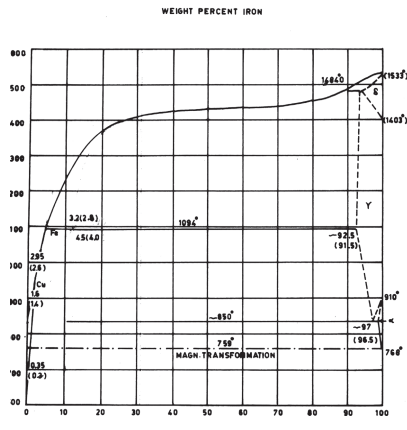
\includegraphics[scale=.7]{images/chapter-3/fig001.jpg}
\caption*{\textit{Behavior of Copper-Iron during reduction (Hansen, Phil Max 1958:581)}}\label{chapter2-fig001}
\end{figure}

\vspace{-.4cm}

The study of many ancient period artifacts of copper from several Chalcolithic sites like Ahar prove beyond doubt the skill of the metal smelters in producing copper from chalcopyrite. The possibility that they incidentally produced magnetic copper cannot be ruled out (see Tripathi 1986: 78, 2001: 67-70, Table ~\ref{table III.1}-\ref{table III.3}). Chalcolithic metal smelters had the knowledge of the use of iron ore as flux for smelting of copper. 

The crucial question is whether these copper smelters were aware of the presence of iron in copper and also that they were producing Cu-Fe alloy \textit{i.e.}, magnetic copper instead of pure copper. We have not studied the recent iron artifacts from the sites of the Ganga Plain to be able to comment whether the copper smelters of this region were aware of the presence of copper in iron ore. Such knowledge could lead to experimentation and understanding of iron smelting technology in due course of time. Alternatively, it is also possible that the metal smiths of the Gangetic plains used limonite or hematite ore, which was more easily available in the Vindhyan ranges. It is quite likely that due to scarcity of copper ore in this region, the artisans experimented with alternative ores and accidentally produced iron. It may be noted that copper objects are very rare in this region in the so-called Chalcolithic period. Bone and stone have been used profusely for tool making with a lower proficiency in dealing with copper working; there is a higher possibility that the artisans picked up iron ores and tried to work with them. In this process of trial and error, they could have accidentally produced iron.

It may be added here that most of the early ironworkers, who had recognised iron as an independent metal, especially is those areas where copper is rarely found, chose to work with low-grade iron ores which get reduced at much lower temperature. Such ores are not worth working with in the modern geological terms. But the ancient workers, including the pre-industrial smelters worked with such low grade ores containing enough calcium and silica. Incidentally, it also acted as a self-fluxing agent. Moorey's statement (op.cit, p. 280) that ``red oxide (haematite) and the hydrated form (limonite) both contain a high proportion of iron and, as they are relatively free from sulphur and phosphorus are easily worked to yield iron. The magnetic oxide (magnetite/leadstone) and the carbonate (siderite/chalybite or spathic ore) are also easily worked". According to him high-grade rich ores are more problematic.

The issue still remains to be investigated in greater detail with regard to the metal smiths of the Vindhya-Kaimur region on the borders of the Ganga Plain. But hematite, magnetite and limonite are available in great abundance in this region that too in the form of nodules and these were used till recently by local smelters. One may ask whether the iron at the earliest levels at sites like Nal-Ka-Tila and Malhar and more recently excavated site of Raipura in the same ore-rich region nearby used such ores. Evidence of use of river sand is also reported from this area. However, what is certain that living in an iron ore-rich area, the tribal and possibly the ancient smelters could somehow produce metallic iron in an otherwise Chalcolithic milieu.

\subsection*{2.II. The Middle Ganga Plain}\label{subsection-5}

\vspace{-.2cm}

The Middle Ganga Plain has emerged as an early center for iron, in recent years. There are important sites of Chalcolithic cultures in the Vindhyan region, Eastern Uttar Pradesh, Bihar and Bengal, generally known as Eastern Chalcolithic culture that have yielded iron objects in this very context. Sites like Kausambi, Koldihwa, Nal-Ka-Tila, and Malhar, Raipura in U.P., Chirand in Bihar, Pandurajar Dhibi, Mangalkot, Mahisdal, Hathigra, Barudih and Bahiri in West Bengal (Map-Fig.~\ref{chapter1-fig001}, \ref{chapter1-fig004}) have produced such evidence in pre-NBP Black-and-Red ware phase. Iron, even though in limited quantity appears in the mid-phase of Chalcolithic period at most of these sites. Mangalkot is an exception, where iron shows up in fairly good amount (16 objects) right from the lowest levels of black and red ware (Dutta 1992: 301). It has been dated by the excavators to ca 1500 BCE. In Bihar, sites like Chirand have yielded iron in the Black-and-Red ware phase, in pre-NBP deposit. Similar situations are met with at sites likes Kausambi near Allahabad and sites like Koldihwa in the Vindhyas in Uttar Pradesh. These levels are datable to 1100-1000 BCE. Recent excavations in the Chandauli, Sonbhadra-Mirzapur area by Tewari, at Nal-Ka-Tila and Malhar (Tewari \textit{et al}. 2002, 2003) and Raipura (Tripathi 2014:1010-1016) have yielded evidence of iron around 1500-1400 BCE. Importantly enough, these sites are located in iron mineral rich zone. There is an extensive evidence of smelting at the site. The tradition of iron working continued in this area till recently. The Agaria community of traditional iron smelters has lived there and has produced iron for generations. It may be noteworthy that (1) this area is located in the heartland of India; (2) the cultural milieu is Chalcolithic; (3) and the dates are much earlier than in the neighbouring countries. This leaves little doubt about this part of the country being one of the earliest iron producing areas therefore an indigenous iron producing centre.

\vspace{-.3cm}

\subsection*{2.III. Rajasthan}\label{subsection-6}

\vspace{-.2cm}

At Noh (District Bharatpur, Rajasthan) bits of iron have been found (as a result of sieving of soil) in the Pre-PGW Black-and-Red ware (BRW, henceforth) levels, also datable to 1300/1200 BCE. It is significant indeed, especially in view of the fact that regular use of iron begins in the very next phase (Painted Grey Ware, PGW) along with a continuing tradition of the BRW pottery. Iron working furnaces are stated to be\newpage present in the earliest PGW yielding levels from Jodhpura in district Jaipur in Rajasthan (Agrawala and Vijai Kumar 1976).

Such evidence provides sufficient ground for the assumption that iron technology developed indigenously at some such place in due course of time. In view of the points raised earlier in connection with the diffusion of iron and the positive evidence of early occurrence of iron in India, we are now on firmer ground to suggest an indigenous origin of iron in India. India being such a vast subcontinent, the exact area of origin of iron remains a difficult issue to resolve. We propose to take a look at such centres below.

\vspace{-.3cm}

\subsection*{2. IV. South India: The Megalithic Culture}\label{subsection-7}

\vspace{-.2cm}

The southern part of the Indian subcontinent is characterized by megalithic burials which are rich in iron artifacts. In the Deccan and the peninsular India an interesting phenomenon is overlap between Neolithic and Megalithic cultures. In most of these parts there is near absence of Chalcolithic culture. The Megalithic culture either follows the Neolithic cultural deposit as at Hallur or most of the megaliths are the earliest cultural deposits. Hallur yielded a date of 13/1200 BCE (without calibration, Nagaraja Rao 1971) from the overlap phase. Other sites like Paiyampalli (see tableIII.7) have yielded $^{14}{\rm C}$ and TL dates which take back the antiquity of Megalithic culture to c. 1400/1300 BCE or even earlier. Special mention may be made here of a site located in the campus of Central University of Hyderabad which has yielded an OSL date ranging from BCE 2700 to1395 (Thomas \textit{et.al.} 2008). However, since it does not fall in general range of $^{14}{\rm C}$ dates it has not been highlighted by the excavator, Prof.~K.~P.~Rao. What is worth noting here is the context of the megaliths in southern India. (1) The megaliths are generally associated with iron (though some megaliths in Tamilnadu are said to be Pre-iron (personal communication, K. Rajan).  (2) The burials are invariably located in mineral rich areas. (3) There is dearth of copper artefacts in the preceding or in the collateral cultural deposits. (4) The megalithic builders appear to be a group of warrior class who needed hunting and war weapons. Under the circumstances, especially seeing the nature of tool typology of the megaliths there appears a possibility that metal workers in Deccan and peninsular India had experimented with available ores in their surrounding area and could successfully extract metallic iron. Even otherwise, iron working in India had long been associated with non-Aryan communities. Though further researches may be necessary to prove the point conclusively but circumstantial evidence does suggest an independent origin of iron in the megalithic zone. The characteristic features of the megalithic cultures with reference to iron will be discusses in greater detail, a little later.

\vspace{-.3cm}

\section*{The Early Iron age Cultures in India}\label{section-3}

\vspace{-.2cm}

The early Iron Age of India is distinguished by the three important ceramic cultures, \textit{viz}. the Painted Grey Ware, the Black-and-Red Ware and the Megalithic cultures in different eco-zones of India. These cultures came into existence immediately after the Chalcolithic period. Factually speaking, many of the cultural traits of the previous period continued to survive even in the succeeding period with the introduction of iron. The archaeological significance of these cultures may be discussed briefly here to give a perspective to the cultural background related to the issue of emergence of iron in India.

\vspace{-.3cm}

\subsection*{3.I. Painted Grey Ware Culture}\label{subsection-8}

\vspace{-.2cm}

The Painted Grey Ware (PGW), a beautiful smooth grey ceramic with black paintings, was first brought to light during the excavations at Ahichchhatra (district Bareilly, U.P.) in 1940-44 (see, Tripathi 1976; 2012). The earliest period at the site belonged to Ochre Coloured Pottery Culture (OCP). A thin deposit of 50 cm characterizes this culture. It is an impoverished culture with a red ware. This ceramic spreads over most of the western Uttar Pradesh, Punjab, Haryana and Rajasthan. It has been associated with the Copper-Hoards, large catches containing heavy tools of nearly pure copper, with a few exceptions which show arsenic alloying. However, the culture came to an end due to violent climatic changes. The pottery with rolled appearance testifies a long exposure to elements or submergence in water. This culture has generally been dated between c.2500-1200 BCE at different sites, thus it is contemporaneous with the Harappan Civilization. After the disappearance of OCP the sites remained deserted for a long time till the next occupants using PGW arrived to settle there. 


A true picture of PGW culture (our zone B) emerged with the excavations at Hastinapur (Lal 1954-55). After Hastinapur excavations, Lal conducted extensive explorations in parts of Ganga and Sutlej Basins.~He brought to light a large number of PGW bearing settlements. Since most of these place names find mention in the epic \textit{Mahabharat}, Lal associated PGW with the \textit{Mahabharat} culture. Interestingly, ancient Hastinapur was the capital of the Pauravas, the heroes of the Great epic. 

The PGW culture has an extensive distribution (Fig \ref{chapter1-fig001}). It has been reported from the Himalayan foothills at Ropar in Punjab in north to Gilund and Ujjain in South, and from Bahawalpur State (in Pakistan) and the Thar Desert of Bikaner in the Vedic Saraswati-Drisadvati basin in the West to Kausambi on the River Yamuna near Allahabad in the east. PGW has been also found outside this zone at sites like Thapli, Kashipur and Purola in the hills of Kumaon-Garhwal in Uttarakhand. An unpainted variety but very similar to PGW in every other respect has been found at Manda in Jammu-Kashmir. Although the culture is generally at home in the plains, as revealed by its distribution map, its recent occurrence in the hilly zones of Kumaon-Garhwal is indeed significant. Since the alluvial plains are devoid of minerals like stones and ores, the culture seems to have made inroads into the hilly tracts for obvious reasons.

The important sites of the PGW culture are Hastinapur, Ahichchhatra Alamgirpur, Allahpur, Atranjikhera, Jakhera, Mathura, Noh, Jodhpura, Roper, Bhagwanpura etc. A close study of the ceramic tradition as well as the cultural material shows a cultural shift from the Indo-Gangetic divide in Sarasvati-Gagghar basin to Ganga-Yamuna \textit{Doab}. In the former zone the sites appear to be a bit earlier in date, at times overlapping with the later phase of the Harappan civilization (1300-1200 BCE). The PGW - both the ceramic and the culture associated with it assumes maturity in the region of Ganga Yamuna Doab. It is in this region that for the first time iron comes to be associated with it.  The iron objects at this stage usually fall in the category of hunting tools like arrowheads, spearheads, points, knife-blades, axes, pins, nails, rods, a pair of tongs from smithy (from Atranjikhera), sickle and rarely ploughshare (Jakhera) have been found, (Table~\ref{table IV.8}). 

The site of Noh (district Bharatpur, Rajasthan), Atranjikhera and Jakhera (both in district Etah, UP) situated close to the mineral rich Agra-Gwalior belt have yielded iron working evidence complete with furnace remains, slag, ash, charcoal and tools like a pair of tongs. Jakhera has yielded a large semicircular slag lump shaped after the furnace-base with pieces of charcoal sticking to it. It provides a good idea about the size and shape of the furnaces that were used there. The excavator of Jakhera has sub-divided the PGW into two periods, i.e. Proto-PGW and PGW cultures on the basis of the nature of the ceramics. The other material remains are nearly identical but for introduction of the PGW in the succeeding phase. The pottery of the earlier period is red instead of grey in colour with identical stroke paintings in black colour like the ones found on the PGW sherds. Sahi has argued a similarity in the ceramic tradition of Jakhera and those found in the hills of the Vindhyan range like Koldihwa, Malhar and Nal Ka Tila, Raipura on the one hand and the Chalcolithic Ahar on the other (Sahi, 1994). If we situate such evidence in the larger perspective of introduction of iron, it is quite significant.

The other ceramics associated with this period include, Red Ware, plain variety of Grey Ware, Black-and-Red Ware without painting, Black Slipped ware. The material culture may be identified with materials like terracotta \textit{ghata} or vase shaped and areca-nut shaped beads (both plain and incised varieties), ball, disc, seals, bangles, gamesmen, and a few animal figurines like bulls, rams, birds and a horse figurine (from Hastinapur). Semi-precious stone beads made with agate, jasper, carnelian, chalcedony etc. also occur along with those of bone and ivory. Kohl sticks of ivory and copper, hairpins, combs, and bangles of horn are other interesting \textit{objects de toiletries}. Copper was used for fashioning ornaments like pendants, bangles, rings etc. and toiletry objects like antimony rods. Other copper objects found in excavations are arrowheads, hooks, chisels, borers, nail-parers, needles, pins and a few pots like bowls. Gold objects, including a sheet of gold has been found from excavations at Jakhera (Sahi, op. cit.). Glass came to be used for the first time with PGW culture. Thus there appears to be a greater degree of skill in the area of pyrotechnology during the PGW period.

Most of the sites of the PGW culture have been excavated on a limited scale, therefore our knowledge about the settlement pattern, especially the structural remains is very limited. However, the thickness of the habitational deposits of the PGW culture varies from a couple of meters to four meters. This shows the long span of the PGW culture. It was from this period onwards that a continuous occupation of sites of the Ganga Plain began. The excavator of Atranjikhera (Gaur 1983) has divided it into three sub-periods demonstrating an evolving cultural trend within this period. Generally, wattle and daub structures, or mud brick houses were in vogue during this period. The site of Jakhera, as an exception, has yielded a couple of large sized baked bricks along with an evidence of a 5 m wide and 0.8 m high protective rampart, a water channel and rammed road. This indicates a well-organized socio-political system in 1000 BCE in the Upper Ganga Plain. Crafts specialization is equally well evidenced with presence of metal working workshops, and glass making activity. Thus with the use of iron, glass, beautiful ceramic tradition and a settled life the PGW culture may be have brought the Ganga Plain to the threshold of urbanization(for details see Tripathi2012). It may be given the credit of laying the foundation of an uninterrupted cultural sequence that is more or less continuous almost till the present day.

\vspace{-.3cm}

\subsection*{3.II. Northern Black Polished Ware Culture}\label{subsection-9}

\vspace{-.2cm}

The PGW culture is followed by the Northern Black Polished Ware Culture (NBP) without any break. Hastinapur is the only exception to it because its occupation ended due to heavy floods in the Ganga. The NBP culture may roughly be dated to c.~700/600-100 BCE with at least two sub-phases designated as Early and Late. However, recent radiocarbon dates have pushed back the antiquity of NBPW by couple of centuries(see Table~\ref{table III.6}). The NBPW period roughly corresponds with the Buddhist period and the period of rise of cities, referred to by many scholars as `second urbanization' of Indian history. The NBP culture also coincides with the rise of the Magadhan Imperialism and its later phase with the Mauryan Empire.~The distribution of the culture extends over five modern states, viz. India, Pakistan, Bangladesh, Nepal and Sri Lanka.

It is during the NBP period that an overall growth in material culture is discernible with introduction of coinage and writing, regular use of baked bricks, defense structures etc. The technological skill shows a marked improvement especially in the field of pyrotechnology, including ceramic technology. The NBPW itself is an expression of high artistry and a highly evolved skill in the kilning and potting techniques with its uniform surface and shining golden, silvery, bluish and blackish colours that has proved to be enigmatic even to the modern scientist and ceramic experts.~It has not been possible for them to unveil the composition used in its surface treatment imparting it the typically unique finish.

This glossy finish or metallic sound has caught the attention of many ceramic experts. A large number of scholars have tried to unravel the enigmatic surface finish of NBP ware, the latest in the series is the recent study by Harding (2004: 34-36). In a nutshell, it may be said that the kilns used by the potters must have been highly efficient with proper mechanism of temperature control. Interestingly iron seems to have played a role in imparting a shine that the surface and colour of NBP has got.  This skill of kilning technique appears to be closely inter-linked with the furnace design exhibiting a temperature control in the iron working. Evidence of carburization, quenching and tempering came into practice during this period. The other noteworthy feature is that it is during this period that the ore rich areas of the country had come to be occupied. Special mention in this regard may be made of the rich ores of Bihar and Odisha. It is in this very zone that the empire of Magadh came to flourish in $6^{\rm th}$ - $5^{\rm th}$ BCE.

\vspace{-.3cm}

\subsection*{3.III. The Pre-NBP Cultures of Middle Ganga Plain}\label{subsection-10}

In the Middle Ganga Plain that is said to be the epicentre of NBPW. A Chalcolithic culture with Black-and-Red Ware (BRW) and/or Black Slipped Ware (BSW) as dominant pottery tradition flourished. As a dominant ceramic before NBPW culture. At several sites of the Middle Ganga Plain the Chalcolithic culture is preceded by a Neolithic cultural horizon. There appears to be an uninterrupted sequence of cultures from the Neolithic to Iron Age right up to the historical period in this zone (our zone E). There is an interaction between the Neolithic-Chalcolithic settlers of the hilly tracts of Vindhya-Kaimur belt and those, which occupied the plains. This Neolithic-Chalcolithic culture identifiable with its typical ceramic tradition like the corded ware (a cord impressed pottery) associated with the burnished Red Ware and Grey Ware and also a cruder variety of BRW extends throughout the Middle Ganga Plain. Some of the important sites of the Culture are Koldihwa-Kakoria in the hills and Chirand, Taradih, Chechar-Kutubpur, Maner, Senuwar and Narhan culture sites and more recently discovered site of Lahuradeva in district Sant Kabir Nagar (Uttar Pradesh). 

In the succeeding Chalcolithic period the pottery of the previous (Neolithic) period continues. However, there are noticeable changes in material remains.~There is an improvement in the surface treatment of ceramics and introduction of copper with the beginning of use of small copper objects like fishhook, wire, needle (at Senuwar). Stone objects like celts, including polished ones, pestle and querns and large number of bone tools are found at most of the sites. At sites away from mineral resources such as Narhan, Sohgaura, Imlidih, Bhunadih, Vaina, Khairadih etc. stone tools are almost missing. Bone tools are used in profusion.

A characteristic feature of this cultural period is growth of agriculture evidenced by the presence of a rich variety of crops. The evidence of rice at Koldihwa in the Vindhyas dates back to $6^{\rm th}$ millennium BCE. Lahuradeva has yielded equally early dates for beginning of agricultural activities. It takes back the antiquity of rice cultivation in the Ganga Plan to $7^{\rm th}$ millennium BCE. Senuwar at the base of Kaimur range and Narhan in the Saryupar plain have yielded millets like \textit{kodon}, pearl millet, chick pea, gram, green gram, field pea, lentil, moth bean, horse gram, grass pea and oil seeds like mustard, sesame etc. Senuwar also yielded barley and wheat in period I dated to 2300/2200-1100 BCE. The animal bones are found in profusion at these sites. Bones of cattle, sheep, goat, deer, stag, pig etc. have been identified. Thus the economy was flourishing with animal husbandry and two crop cultivation. Intra-regional contacts are indicated by similarity in ceramic tradition from the hilly zones of Vindhy-Kaimur to the plains of river Ganga and its tributaries.

It is in this milieu that iron was introduced in this zone. Iron has been reported from sites like Koldihwa in the Vindhyas. More recently sites like Raipura and Latifshah, yielding valuable evidence on iron working  have been excavated. The two sites are located in the same Vindhyan area as Malhar and Raja Nal-Ka-Tila. One may say that they are in the same league, culturally as well as chronologically. These sites have yielded iron in the earlier half of the $2^{\rm nd}$ millennium BCE. The calibrated dates of Raipura range between 1932-1438 cal BC and 1867-1848 cal BC from lower strata and 1257-1234 cal BC from mid-iron yielding levels (Table~\ref{table III.10}, \ref{table III.11}). There are a good number of sites in the Middle and Lower Ganga Plains that have yielded a similar evidence of occurrence of iron right in the Chalcolithic context (see Zone E, below). Generally the only reason for distinguishing the two cultural horizons is the emergence of iron. The material culture hardly shows much change with the introduction of iron. The main pottery of this period continues to be a BRW with white stroke paintings, Black Slipped Ware of both plain and painted varieties (typologically different from the BSW of the succeeding NBPW period), a fine Black Ware, Red Ware and a Grey Ware both, burnished.  The other finds reported from this period are terracotta beads, discs, balls, a rich variety of bone points and arrowheads of both tanged and socketed types. Terracotta animal and bird figurines also occur. It may be mentioned here that Narhan does not yield even a single stone object in pre-NBP period. This evidence is also supported by a substantive number of sites of Saryupar plain. Because of this Singh (1994) labels this group of sites as Narhan Culture. The house remains of this culture consist of wattle and daub houses having plastered screen walls of reed and bamboo. Most of these sites are dated between c. 1400/1300 and 800 BCE.  The iron objects are reported right from the earliest period. Period I at Narhan yielded only a point and an indeterminate iron object. The number grows to 42 in the succeeding period. 

This cultural tradition continues up to Bengal. There are a number of sites in Bengal, such as Pandu Rajar Dhibi, Hatigra, Mangalkot etc. that have yielded iron in a Chalcolithic milieu. The term \textit{Ferro-Chalcolithic} has been suggested by Chattopadhya (2004) for such cultural levels. Wattle and daub houses, postholes, stone and bone tools, a few copper objects are the other findings reported by the excavators. At some of the sites, such as Pandu Rajar Dhibi, evidence of metalworking has also been unearthed. Radiocarbon determinations date this cultural phase to c. 1200/1100-800 BCE. But the Iron Age sites of Bengal have been dated to 1100-1000 BCE ($^{14}{\rm C}$ 950 BCE, Mangalkot and 990 BCE from Pandu Rajar Dhibi, uncalibrated dates, Datta 1998: 36-43). Mangalkot has yielded iron objects in good number and right from the earliest phase. 

\subsection*{3.IV. The Megalithic Cultures of Vidarbha and\\ Peninsular India}\label{subsection-11}

The southern part of the Indian subcontinent beyond the Vindhyan ranges is dotted with burials using huge stones that have earned them the title of Megalithic culture. These burials are distributed in the hilly tracts from the Vindhyan ranges south of the Ganga Plains to the peninsular India in the deep south. They have a wide distribution both in time and space. The Megalithic cultures of Karnataka, Andhra and Tamilnadu overlap with the Neolithic cultures and continue right up to the Historical times. In certain parts Megalithic burial is still practiced as the mode of last rites. Certain $^{14}{\rm C}$ and TL dates have recently pushed back the antiquity of Megalithic culture from c. 1400/1300 BCE to the beginning of the second millennium BCE. As noted above, the megalithic burials exposed at Gachibowli in the campus of the Central University of Hyderabad have OSL-TL dates going back to 2800-2000 BCE (Thomas \textit{et.al.}, op.cit). However, we need to work further and procure more reliable scientific dates to decide the chronology of south Indian megaliths. A phase of iron free megaliths followed by iron bearing burials in Tamilnadu (Rajan, personal communication) suggests that the megalithic builders introduced use of iron in the peninsular India. Intensive archaeological investigations being carried out in the region is likely to throw more light on the subject in near future.

In most of the southern India there is a near absence of Chalcolithic culture. The Neolithic culture overlaps with the iron bearing Megalithic culture. Towards the end of the Neolithic period use of copper, albeit at a minimal level begins. The iron using megalithic folk takes over the region in a big way occupying a certain ecological zone of southern India. Sites like Paiyampalli and Hallur with a date of c. 1300-1200 BCE are good examples. It may be noted that most of these burial sites are located in the mineral rich hilly zones. The settlement sites are found closer to streams, rivulets or some such water bodies, for obvious reasons. Most of our knowledge about this culture is based on the burial remains that are rich in grave-goods. The habitation sites provide information about their economy and life-style. The settlements in the fertile land in the Krishna-Kaveri and Godavari basins are richer in agricultural remains. Even a wet crop like rice was grown in these areas while sites away from the river valleys such as in the Deccan yield evidence of coarser grains like millets, grams, pulses, oil seeds and cotton. A special variety of BRW was in use during the period. 

Ecology seems to have played a strong role in shaping the culture of the megalith builders. No large-scale agriculture was possible in the predominantly hilly zones where this culture is more at home. Therefore, they seem to have taken to an alternative means of livelihood. It is also reflected is the tool typology of megaliths (Table~\ref{4. IV	}). Sickles and hoe are the only agricultural implements that occur only as a small percentage (2-3\%) of the total number of iron objects. Most of the iron objects fall in the category of hunting and weapons of offence such as spears, arrowheads, axes, javelins, daggers, choppers, swords, tridents etc. An in-depth study of tool-typology and their metallurgy has been undertaken by Sasisekaran (2004).  There are household objects, such as utensils, (bowls, pans, ladles), lamps, knives, nails, hooks etc. and artisan's tools like chisels etc. A number of megalithic burials have yielded horse bits like cheek-bars. Special mention may be made here of sites like Kunnattur, Sanur, Adichanallur, Brahmagiri. Takalghat (in the Vidarbha region) has yielded a full-fledged horse burial.

A close study of the tool repertoire as well as the cultural setting and material remains of the Megalithic culture - all point towards a war-based economy. It must have been a chiefdom society (Deo and Jamkhedkar 1982). A grave at Adichanallur has yielded a gold diadem; only a few graves have got gold ornaments in them while the rest of them contain only ordinary objects of lesser value. This clearly suggests a social hierarchy, and some kind of chiefdom based political system.

The flimsy settlements with thatched roofed circular houses with lime plastered floors are hardly in keeping with the affluence that is otherwise displayed by the grave goods. Gold, silver ornaments, beads of semi-precious stones, beautifully crafted cropper objects in some of the burials reflect the mastery of the craftsmen. Many sites like Naikund in Vidarbh and Guttur in Tamilnadu have yielded furnace remains indicating a local smelting-forging of metals at such sites. Kudumnal is another site which is of great significance from the point of view of iron technology and its chronology. 

Crucible steel is an innovation achieved by the iron workers of southern India. According to recent $^{14}{\rm C}$ dates from Tamilnadu crucible steel started to be produced somewhere around $4^{\rm th}$-$5^{\rm th}$ BCE and continued to be in great demand till early parts of twentieth century. Wootz steel locally known as \textit{ukku} attracted West and Central Asian traders who were flocking Deccan and southern Indian ports in large numbers. Beautiful swords made with wootz steel having an intriguing watering pattern on the surface were famous all over the world as Damascus steel. Pliny in \textit{Natural History, The Encyclopedia of the Roman Empire} mentions about import of iron and steel from Seres identified with the Cheras of south India. The Sangam literature also refers to a brisk trade with the Yavanas in the early centuries of the Common Era. Excavations like Arikamedu have shown presence of Roman artifacts confirming such interactions. The \textit{Periplus of Erythrian} Sea has also mentioned the Seres (Cheras) shipping variety of commodities from the western coast like Muziri on the Malabar Coast (Schoff 1912). We also hear about Seric iron that is significant in the present context (for detail see Srinivasan and Ranganathan, 2004). Although the south Indian centres of crucible steel are well known, literary accounts pertaining to early centuries of Christian era attest to presence of sword making centers in several other parts of India as well (Tripathi, 2007: 403-426). 

However, a question that has frequently been raised is the impoverished looking economic status of the settlements despite their being so rich in precious objects. We may hazard a guess in this connection. It is apparent that the priority of the Megalithic builders seems to be wars and marauding (see Tripathi 2001: 232-33) than developing townships. Their technological skill was directed towards manufacturing objects of offence. Thus the case of megalithic culture seems to be different than the other regions in the river valleys and alluvial plains discussed earlier. They seemed to have maintained an independent existence in secluded but mineral rich zones, exploiting it to its full potentials and eked a living out of this.

The recent analysis of iron objects from Mahurjhari show knowledge of steeling in this region in ninth century BCE (Deshpande 2010: 636-639). This fact has been corroborated further by recent excavations in parts of Tamilnadu (Rajan et.al.2021:57-86). Production of this type of steely iron could have been achieved only with a long experience in the field of metallurgy. There are $^{14}{\rm C}$ and TL dates take the antiquity of iron in peninsular India to 1400 BCE.  Thus we come across radiocarbon dates ranging from first half to middle of the second millennium BCE from several parts of the Indian subcontinent.

This brief description of the cultures of second-first millennium BCE provides us an insight into the nature and types of development and the pattern of growth of cultures in different eco-zones of the subcontinent. In the specific context of the development of iron technology, we may now explore the possibility of finding the precise centers of early iron working in the subcontinent.

\vspace{-.2cm}

\section*{Early Centers of Iron in India}\label{chapter3-section-4}

With this, we come to the difficult juncture of identifying the earliest centers of iron in the country. In India it was only around 600-500 BCE that truly inter-regional contacts and some kind of cultural homogeneity embracing different and often distant regions seem to have developed at a perceptible scale. The period before 600 BCE is characterized by the multiple cultures occupying limited geographical regions. The few inter-regional contacts were confined to contiguous regions particularly where any physical barriers did not hamper movements.~It was in this context that first smelted iron occurred,~not in one particular region but in quite a few of them and often in widely differing cultural contexts. Two questions naturally arise here: 
\begin{itemize}
\item[1.] Which is the region that has a greater claim for having ushered in the metallurgy of iron?


\item[2.] Was there only one center where it emerged and diffused to other centers or conversely, there were more than one center where iron smelting might have emerged independently? It would be helpful to closely examine each region separately. Six cultural zones, discussed below briefly, could be discerned in accordance with the cultural and geographical divisions (Fig.~\ref{chapter1-fig002}).

%~ \item[2.] Was there only one center where it emerged and diffused to other centers or conversely, there were more than one center where iron smelting might have emerged independently? It would be helpful to closely examine each region separately. Six cultural zones, discussed below briefly, could be discerned in accordance with the cultural and geographical divisions (Fig \ref{chapter1-fig002}).

\end{itemize}

\vspace{-.3cm}

\subsubsection*{\textit{Zone A:}}

\vspace{-.2cm}

In this zone, consisting of North-West Frontier provinces of Pakistan and the adjoining parts of Kashmir, a large number of cairn burials have been located. In Baluchistan as discussed above, at Ziwanri, Take Dap, Moghal Ghundai, Gatti, Zangian etc., nearly 200 cairns were plotted and some of them briefly excavated by Stein (1937) and Mockler (1943, 1876). The burials do not conform to any uniform pattern - neither in grave goods nor in burial practices. They contain a variety of pottery belonging to diverse types. Even chronologically they do not belong to any specific date bracket. Some graves have been opened a number of times making it difficult to date them safely. Iron objects like arrowheads, spearheads have been found along with ornamental objects of copper, bronze and silver with pottery and bones.

At Pirak in the Kachchi plains of Baluchistan, a unique culture has been discovered, having no parallels in the vicinity (Jarrige and Enault, 1973). A total of 11 layers were discerned there. Iron appears in layer 6 accompanied by a grey coloured pottery which appeared for the first time at this stage. It is roughly datable to 1000 or 900 BCE. Agrawal, on the basis of a large number of consistent $^{14}{\rm C}$ dates, suggests 900/800 BCE for the inception of iron at the site.

In the Gandhara Grave Culture Ghaligai, Katelai, Butkara, Timargarh etc. in Swat Valley (Pakistan) iron comes from several graves. The related stratigraphy and chronology is controversial (Dani 1967, Stacul 1969). Iron is associated here with a new kind of dark grey pottery. The iron objects consist of arrowheads, spearheads, nails, finger rings and horse cheek bars. $^{14}{\rm C}$ dates from these levels range between 1200 BCE and 800/700 BCE.

At Burzhom and Gufkral in Jammu-Kashmir iron has been detected in burials. Little is published to give us an idea of cultural material, though the graves were earlier designated as Buddhist by the excavator (Sharma 1979-80, 1992). The iron yielding levels at Gufkral have been dated to 1900 by $^{14}{\rm C}$ recently. However, definite conclusions cannot be derived till further details are available and the reports are published providing us details about the precise nature and circumstances of occurrence of iron there. However, these early dates from iron bearing levels in this region push back the chronology of iron by several centuries. This calls for a serious consideration by scholars about problems related to the advent of iron in the subcontinent.

\vspace{-.4cm}

\subsubsection*{\textit{Zone B:}}

\vspace{-.2cm}

Away from the hilly tracts of the above zone, we come across the iron bearing culture of Doab, i.e. Painted Grey Ware Culture (Tripathi 1976; 2012) which is centred in the valleys of the rivers Saraswati, Drisadvati, Ganga and Yamuna. Unlike Zone A, no burials are reported from this culture. Asian exception to this however, the site of Abhaipur (Dist. Pilibhit, U.P) yielded two barials one of an adult \& one of a child Bhagwanpura also yielded Duraials, (see Tripathi 2012; 276). Perhaps cremation was generally practised by the people. Iron comes from regular habitats. The culture appears to have a simple agrarian village economy with mud or mud brick houses. Glass was used for the first time in this area at PGW level, with iron working which starts at many places, especially in Doab from the very beginning of this culture. The evidence of Jakhera (district Etah, U.P.), however, seems to hint at a more urbanized trait, with a better-evolved and more affluent socio-economic condition, (Sahi 1978). There is evidence of well-rammed roads, man-made water channels, and rich antiquities including a variety of gold objects. As noted above, it may safely be said that this culture brought \textit{Doab} to the threshold of urbanization. This may broadly be dated to the beginning of the $1^{\rm st}$ millennium BCE. Though a higher antiquity has been claimed for PGW (Gaur 1983, Lal 1954-55), 1000 BCE appears quite logical, especially on the combined testimony of $^{14}{\rm C}$ dates and archeological evidence (Tripathi 1987.). Only a solitary date of 1025$\pm$110 BCE from Atranjikhera goes into $2^{\rm nd}$ millennium BCE but places like Bhagwanpura, which show an overlap with Late Harappan culture, may be of somewhat greater antiquity.

\vspace{-.3cm}

\subsubsection*{\textit{Zone C:}}

\vspace{-.2cm}

Over a distance of nearly hundred km, from Kausambi in the west to Rajghat (district Varanasi) in the east, we do not come across any contemporary culture. At Ayodhya, Sravasti etc. we have come across ancient habitations but they do not date beyond 700/800 BCE. In Rajghat, we come across a Black-and-Red Ware culture at its earliest phase, which yields iron right from the beginning. The intermediate areas of eastern U.P., Bihar and Bengal are known to be using iron roughly in 1500-1000 BCE. Recent evidence of early use of iron has been brought forth by excavations at sites like Raipura, Raja-Nal-Ka-Tila and Malhar in district Chandauli and Sonbhadra in the Vidhyan plateau quite close to Varanasi. The evidence is further substantiated now by Jhusi (Allahabad) and Lahuradeva (Sant Kabir Nagar). The radiometric dates of 1800-1500 BCE have pushed back the origin of iron several centuries back. Other important sites of this zone are Narhan, Chirand, Vaisali, Sonpur, Rajgir, Kumrahar, Pandu-Rajar-Dhibi, Mahisdal, Mangalkot etc. This phase not only shows a contemporaneity with zone B but also possesses many common cultural components seen in beads, bangles, nature of settlements etc. However, the pottery traditions are quite different. This region generally had an underlying Chalcolithic level, before the incoming of iron. To be precise, iron in this region is introduced in a Chalcolithic milieu. The cultural traits continued to be unchanged for quite some time even after the advent of iron. Sites like Khairadih yielded three furnaces in a row (Fig.~5C; 7) in a area which can be termed as workshop area (Tripathi 2018: 70-80).

\vspace{-.3cm}

\subsubsection*{\textit{Zone D:}}

\vspace{-.2cm}

This cultural and ecological zone, consisting of the modern states of Madhya Pradesh and South Eastern Rajasthan and adjacent areas of Maharashtra is separated from Zone C by the Vindhya-Kaimur and Aravalli ranges. Hegde had explored the area around Arawalli hill for metal working. He had tried to reconstruct the smelting activity in form of a furnace at Dhatwa which is located in an ore rich area (Fig.~5B). The Deccan area is rich in ore deposits and has a plethora of Chalcolithic cultures that precede the iron bearing strata. This area is known for its richness in copper-bronze objects from the Chalcolithic period onwards. The main ceramic tradition of this region is the Black-and-Red Ware like that of the Zone C but culturally speaking, and even in the shape and texture of pottery, it is quite different from the above. The map shows them under the same sign but a spatial gap is evident. Key sites of this zone are Eran, Kayatha, Nagda, Prakash, Bahal etc. The Eran Chalcolithic level is dated to 1300 BCE (discussed above) and is shown to be the earliest iron using culture. At Ahar, as discussed earlier, iron reportedly is present in the Chalcolithic level itself, which is $^{14}{\rm C}$ dated to 1600-1400/1300 BCE.  Eran was dated early because of its affinity and continuity with Chalcolithic phase which yielded two $^{14}{\rm C}$ dates of 1300 BCE and 1000 BCE from that level. As stated earlier, the subsequent excavations at Eran do not support an early date any longer. Other iron bearing sites mentioned above have been dated roughly to 700/600 BCE as they all show a gap between the Chalcolithic and iron bearing levels.

\vspace{-.3cm}

\subsubsection*{\textit{Zone E:}}

\vspace{-.2cm}


The megalithic burials of Vidarbh in Maharashtra have yielded evidence of great significance in connection with iron. Excavations conducted at Takalghat ­Khapa, Mahurjhari, Junapani, Naikund etc. have yielded iron at the earliest levels. Both habitation sites and burials thereof have been excavated, revealing pottery of a special type and objects like sword, spearhead, arrowhead, ladle, chisel, axe, spike, fish-hook, horse bit, bangle etc. Deo dates them to 800 BCE (Deo and Jamkhedkar 1982). But recently much earlier $^{14}{\rm C}$ dates have been brought forth pushing the antiquity of Vidarbha megaliths by a couple of centuries (Table~\ref{table III.7}). The Naikund excavation has also yielded an iron-smelting furnace, complete with tuyeres, slag and brick tiles used in its construction (Fig.~\ref{chapter-3-fig5abc}A).

%~ The megalithic burials of Vidarbh in Maharashtra have yielded evidence of great significance in connection with iron. Excavations conducted at Takalghat-­Khapa, Mahurjhari, Junapani, Naikund etc. have yielded iron at the earliest levels. Both habitation sites and burials thereof have been excavated, revealing pottery of a special type and objects like sword, spearhead, arrowhead, ladle, chisel, axe, spike, fish-hook, horse bit, bangle etc. Deo dates them to 800 BCE (Deo and Jamkhedkar 1982). But recently much earlier $^{14}{\rm C}$ dates have been brought forth pushing the antiquity of Vidarbha megaliths by a couple of centuries (Table~\ref{table IV.7} ????table 7 not present in chapter 4 please check it???????). The Naikund excavation has also yielded an iron-smelting furnace, complete with tuyeres, slag and brick tiles used in its construction (Fig.~5.~A).


\vspace{-.3cm}

\subsubsection*{\textit{Zone F:}}

\vspace{-.2cm}

A large number of megaliths have been brought to light from the peninsular India indicating a variety of megalithic burial practices (Sundara 1975). A typical Black-and-Red ware characterises them. They are rich in iron and are $^{14}{\rm C}$ dated to 1100 BCE at Hallur in its neolithic - megalithic overlap phase. Recent TL dates from Kumaranhalli, Tadkanhalli etc. range between 1440 BCE and 1130 BCE. The megalithic burials in the campus of Hyderabad University have yielded OSL and TL dates around 2000 BCE which are far the earliest dates for iron in South India. Future work with more reliable  scientifically  dated megalithic sites may lead to review of existing scenario on Iron Age in South India\endnote{Investigations being carried out in different parts of Tamilnadu have yielded valuable evidence on iron and high carbon steel making from a much earlier date than hitherto believed. Special mention may be made here of Iron Age grave at Thelunganur in Salem district yielding AMS date of 1334BCE and cal 2742 BCE. A sword of ultra high carbon steel (1.2\%) has been reported from that grave.(For details see K. Rajan et.al 2021:57-86).}.

\begin{figure}[H]
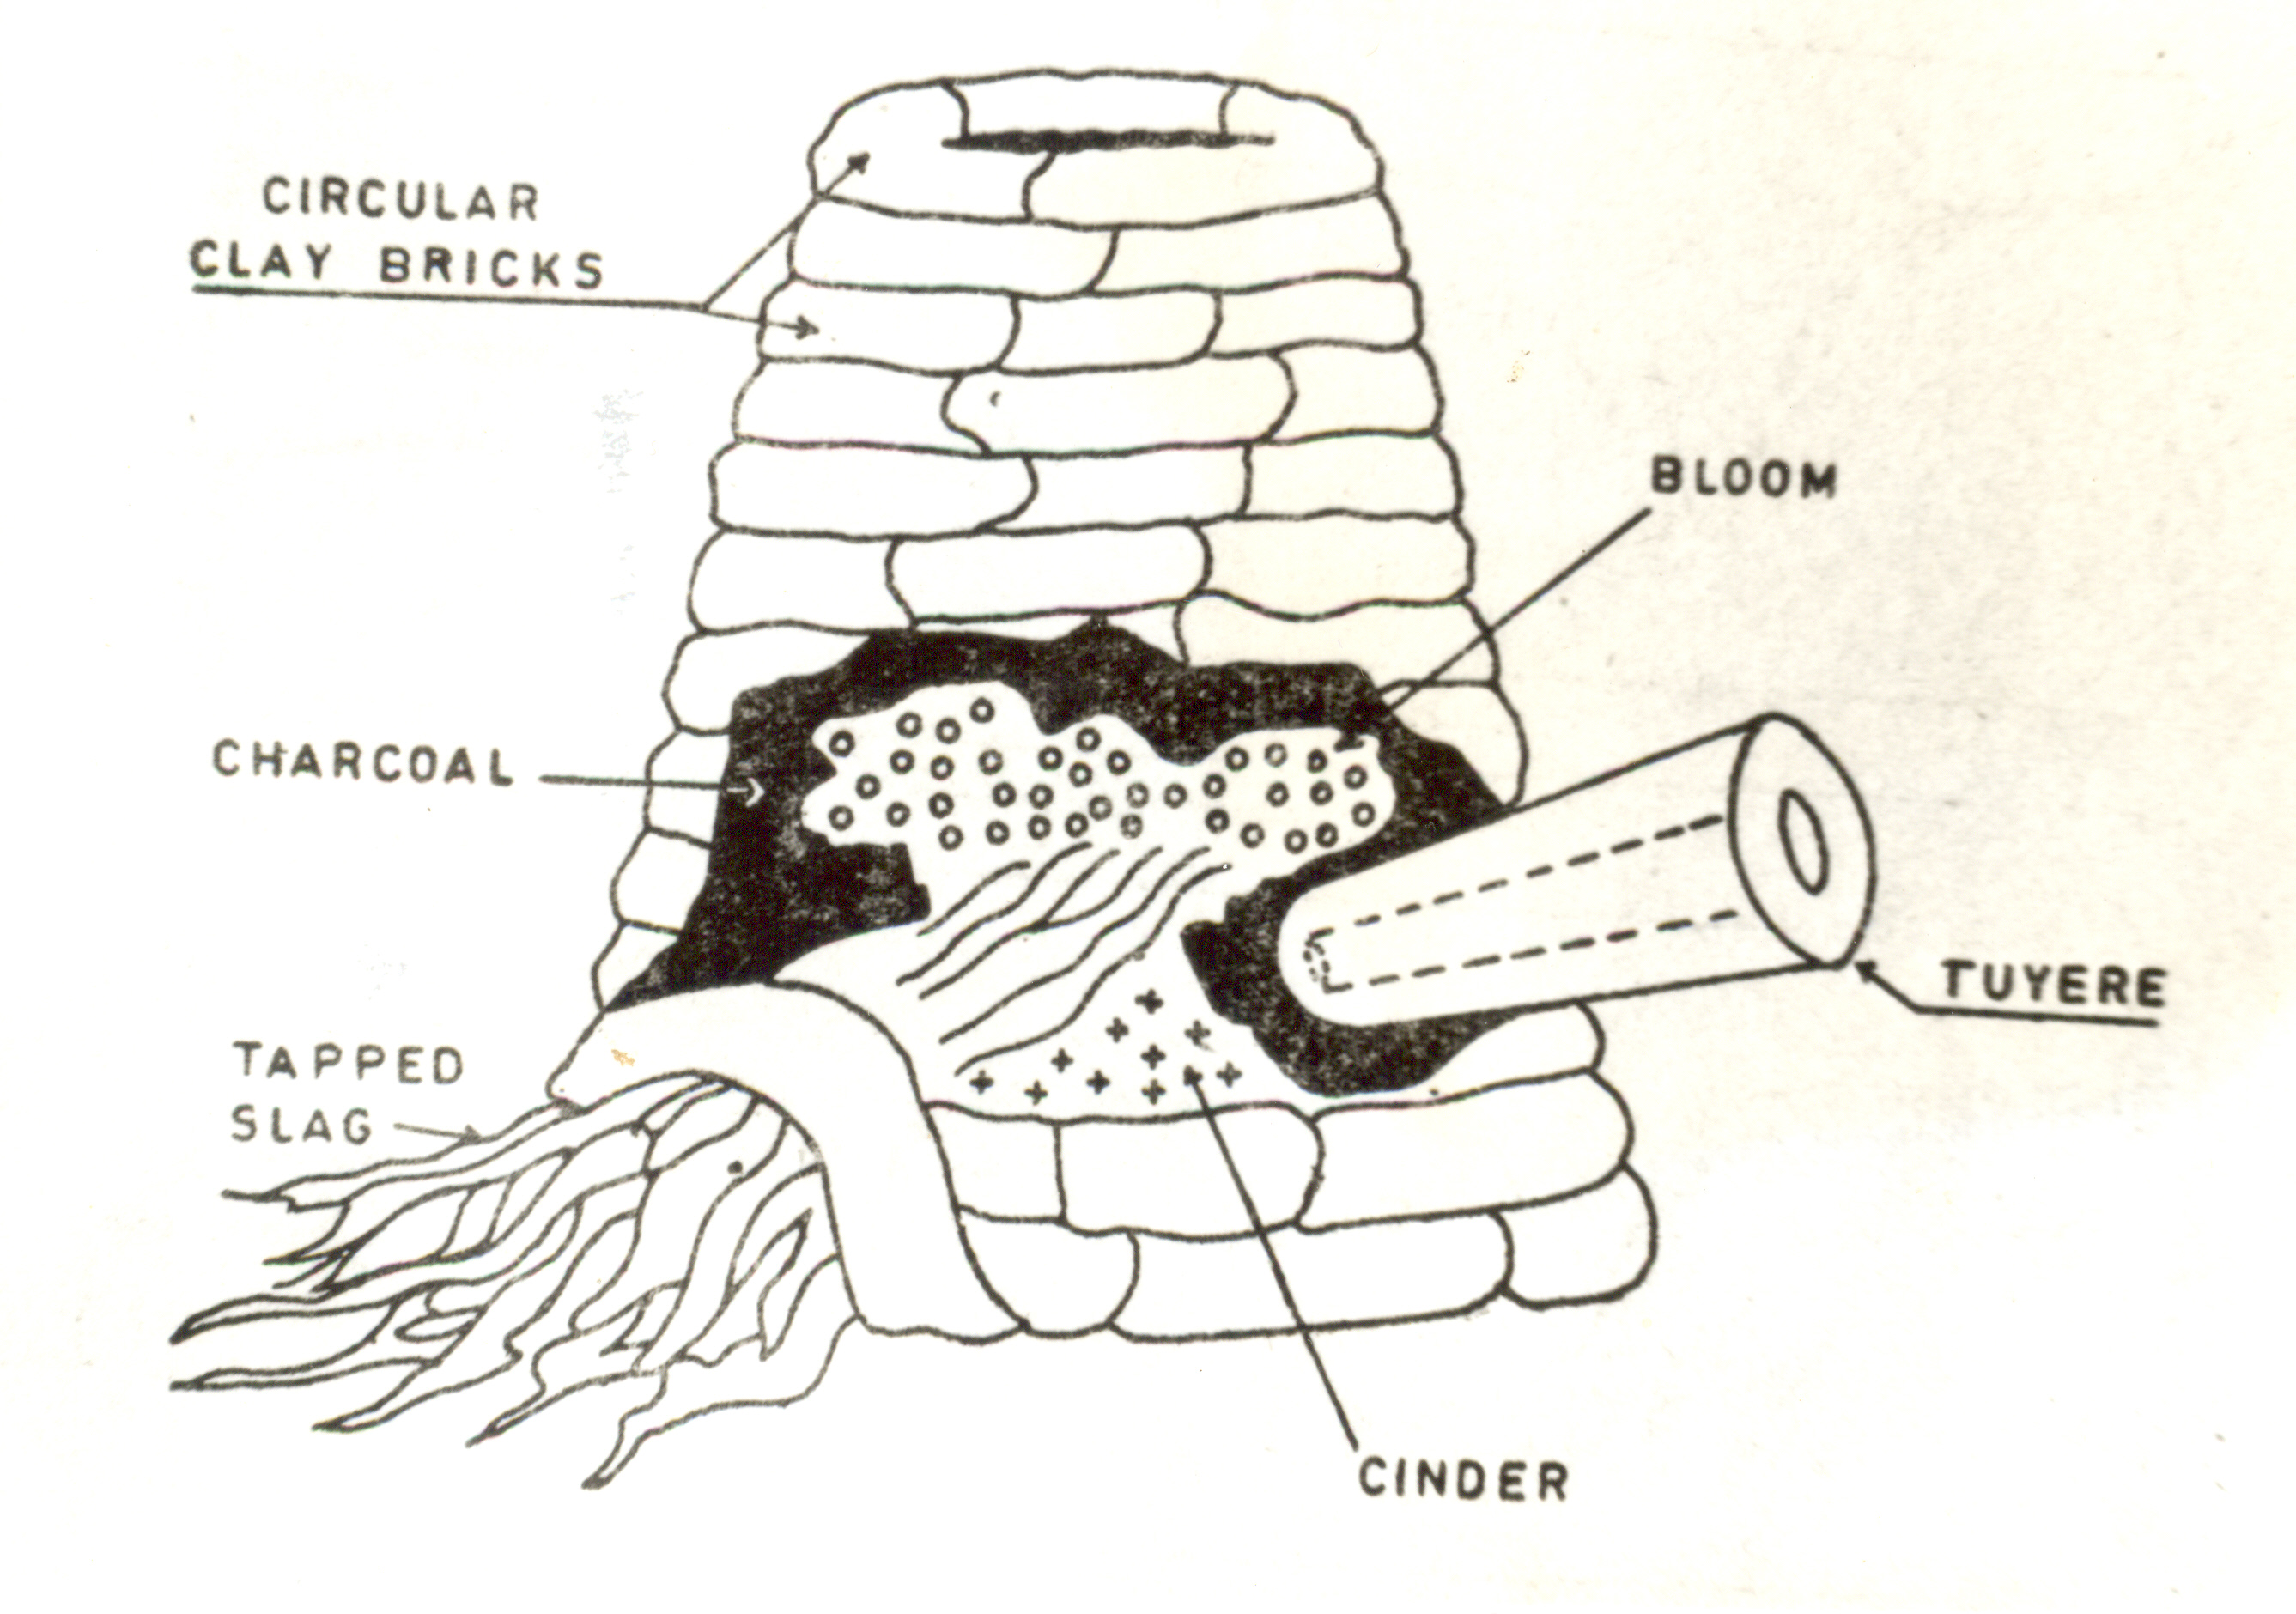
\includegraphics[scale=.65]{images/chapter-3/fig002a.jpg}\label{chapter-3-fig5a}

\vspace{-.3cm}

\caption*{\textit{Megalithic Naikund furnaee}}
\end{figure}

\vspace{-.5cm}

\begin{figure}[H]
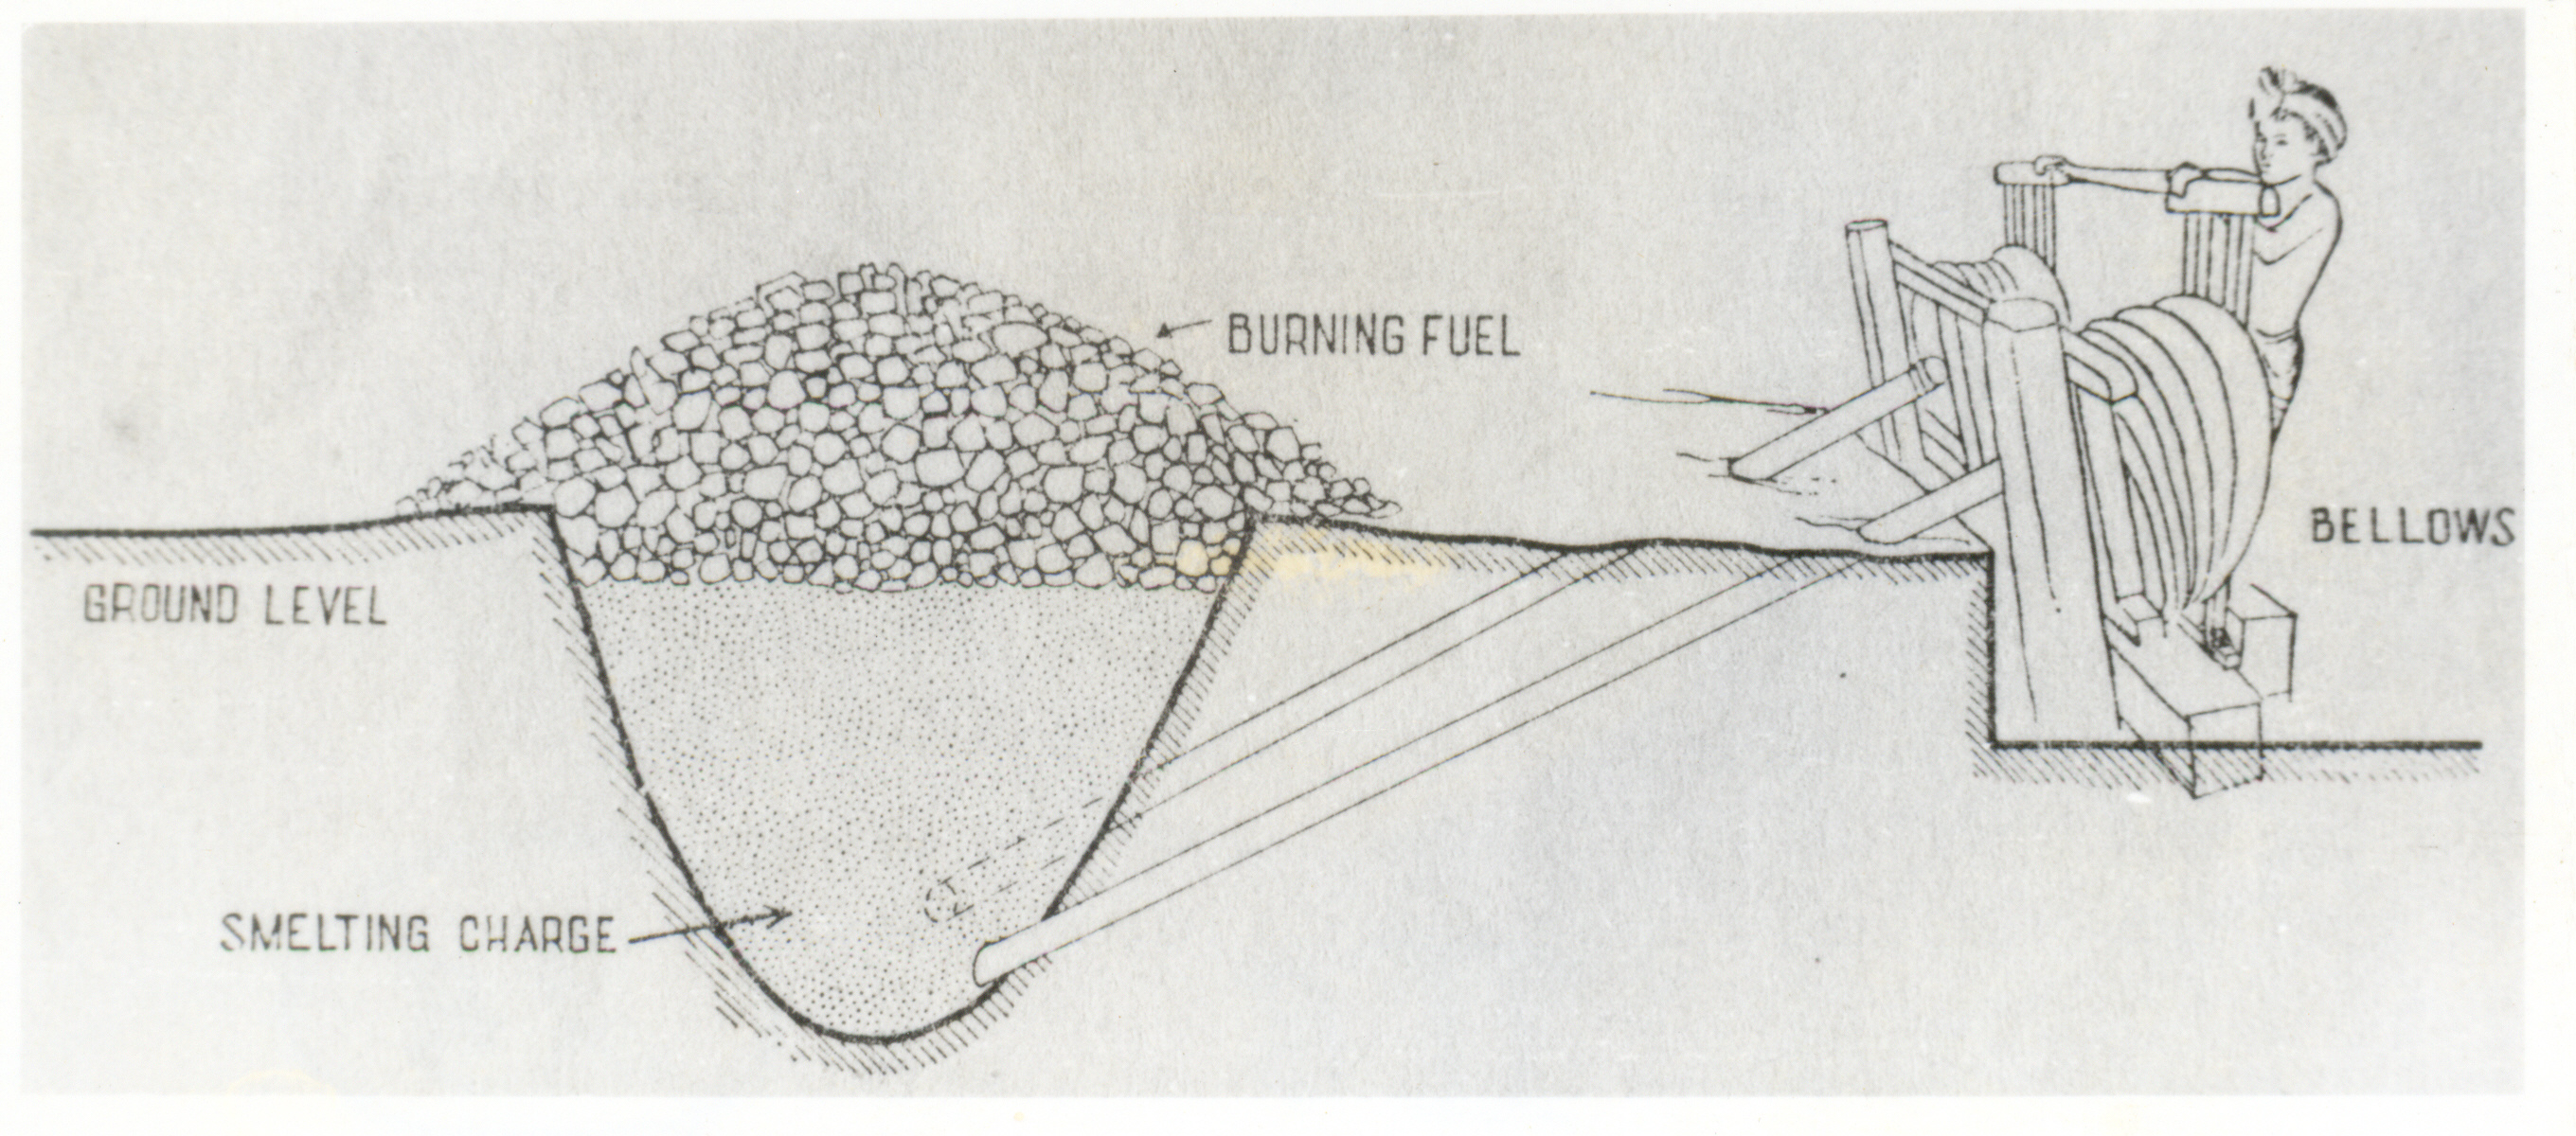
\includegraphics[scale=.85]{images/chapter-3/fig002b.jpg}\label{chapter-3-fig5b}
\end{figure}
\begin{figure}[H]
\setcounter{figure}{4}
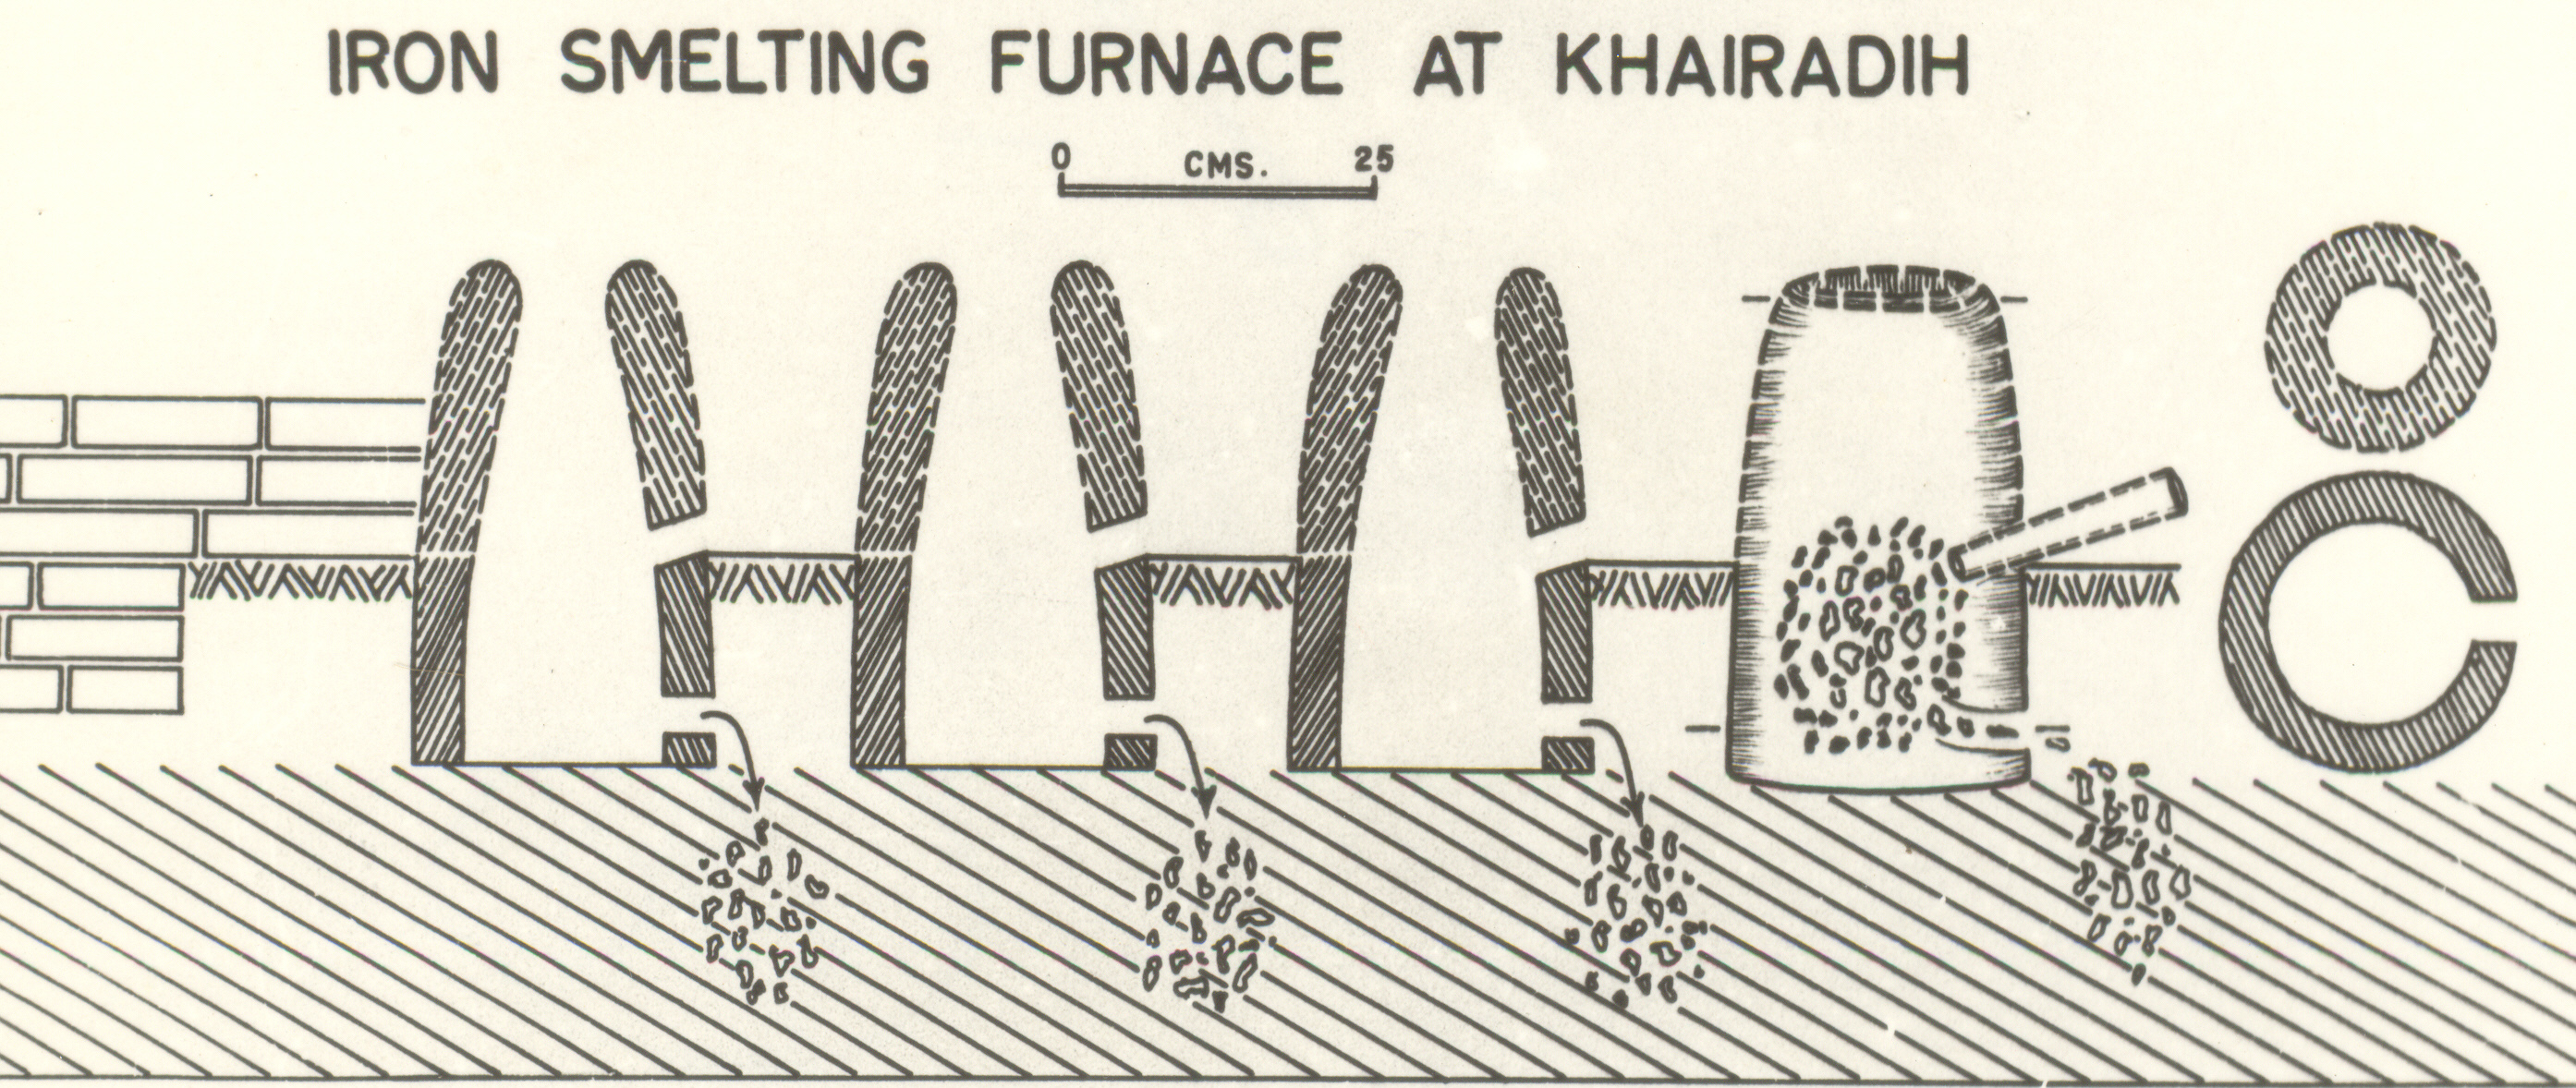
\includegraphics[scale=.85]{images/chapter-3/fig002c.jpg}\label{chapter-3-fig5c}

\vspace{-.2cm}

\caption{A, B, C \textit{Iron-smelting furnaces (reconstructed ancient furnaces)}}\label{chapter-3-fig5abc}
\end{figure}

\vspace{-.7cm}

\section*{Discussion: A Multi-Centred and Indigenous Origin of Iron in India}\label{chapter3-section-5}

Notwithstanding the vague similarities here and there the regions mentioned above largely represent separate cultural groups with prominent individualistic traits. From the above region-wise study, it appears that there is a consistent and well recognised occurrence of iron roughly around 1500-1000 BCE nearly in all the regions. Earlier the PGW was said to be the first culture, which brought iron in India (Tripathi 1976; 2012). Though occurrence of iron at Hallur in 1100 BCE posed a problem for archaeologists way back in the year 1970 – both because of its context as well as dating. But since then we have large number of early dates from large number of sites. Thus (1) we have to push back the antiquity of iron in India in light of fresh evidence. (2) More than one cultural zone in India may be attributed for an independent introduction of iron in the subcontinent.
{\setcounter{table}{0}
\renewcommand{\thetable}{III.\arabic{table}}
{\fontsize{7}{8}\selectfont\begin{longtable}{|p{1.3cm}|p{2cm}|p{.9cm}|p{2cm}|p{1.3cm}|}
\caption{{\fontsize{9}{11}\selectfont (A) Some Recent $^{14}{\rm C}$ Dates of Early Iron Age}}\label{table III.1(A)}\\
\hline
\textbf{Site} & \textbf{Lab-ref.} & \textbf{Date BP} & \textbf{Date cal BC} & \textbf{Pub.ref.}\\
\hline
\endfirsthead
%\multicolumn{4}{c}%
%{\tablename\ \thetable\ -- \textit{}} \\
\hline
%\textbf{Site} & \textbf{Lab-ref.} & \textbf{Date BP} & \textbf{Date cal BC} & \textbf{Pub.ref.}\\
%\hline
\endhead
\hline 
 %\multicolumn{4}{c}{} \\
\endfoot
\hline
\endlastfoot
Raja\par Nala-ka-tila (Sonbhadra)& PRL-2047 &  2890+80 & 1118 (963) 859 1423(1307)1144 & Tewari {\it et.al.} 2000:93.\\
 & PRL-2049 & 3050 + 90& 1196-1188 &   \\
 Malhar \hbox{(Chandauli)} & BS-1633 BS-1593 (Pit sealed by Layer No.(3)) &3450+90 2540+90 & Stuiver and Reimer 1993* 1882 (1743) 1639 2012 (1882, 1836, 1834) 1742 & Tewari {\it et.al.} 2000:88 \\
Dadupur \hbox{(Lucknow)} & BS-1822 BS-1759 BS-1825: (Pit sealed by Layer No. (12)) & 3270+80 3380+160 3430+90 &Stuiver and Reimer 1993* 1679 (1522) 1442 1882 (1685) 1465  1739 (1706) 1695 & Tewari {\it et.al.} 2002:111.\\
Lahuradewa Sant Kabir Nagar & BS-1939 & 2940+100 & Stuiver and Reimer 1993* & (Tewari {\it et.al.} 2002a:57)\\
Jhusi Allahabad, & PRL-2077 &2820+80 &Suuiver and Reimer 1993* 1107 (973, 956, 941) 844 &Tewari {\it et.al.} 2002:111. \\
Komaranhalli Karnataka (TL dates) & PRL-46 PRL-47 \par PRL-49 PRL-50 & &1320 400 1380 300 1130 500 1140 290 & Deo 1991:193\\
Veerampura Andhra Pradesh & PRL-728 PRL-730 & & 620140 1200 140 &Deo 1991:193 \\
Vidarbha, Maharastra & PRL-1361 &2940+160 & 1393 (1205, 1205, 1188, 1181, 1149, 1144, 1129) 917 & Unpublished information from the excavator \\
& PRL-1452& \hbox{3080$\pm$120}& 1490 (1381, 1334, 1321) 1133 & \\
&PRL-1456 & \hbox{2820$\pm$100} & 1185 (973, 956, 941) 834 & \\
Gufkral (Jammu \& Kashmir) & & & 1550-1300 (Uncal)& Sharma, 1992:64-67\\
\end{longtable}}}


It was earlier assumed that most PGW habitations begin with iron but on more westerly sites e.g. Rajasthan, Haryana (Bhagwanpura where it overlaps with late Harappan culture) and Punjab (Ropar) no iron is reported along with this culture. Presumably, there was no iron in the earlier phase of PGW as clear from the evidence of the above sites (Tripathi 1997); it is hard to understand the mechanism of the dispersal and know-how of iron metallurgy on the more easterly PGW sites in c. 1100/1000 BCE. Here attention may be drawn to the very interesting piece of evidence from Noh, referred to above. It is possible to deduce from the evidence that some kind of accidental discovery of bits of iron was made as a result of such an appearance of smelted iron, essentially as a by-product of copper working. What must have followed as a natural corollary was the recognition of iron as a metal in its own rights and its subsequent exploitation.

The chronology of iron in the heartland of India has been pushed back by several centuries with recent discovery of early iron using sites in the Ganga plains, Table~\ref{table III.1(A)}.

Several sites in the eastern parts of the Vindhyas, Raja Nal Ka Tila and Malhar and subsequently Raipura and Latifshah in the neighbourhood of  Varanasi have yielded $2^{\rm nd}$ millennium BCE dates (Tewari 2003, Table~\ref{table III.2} \& ~\ref{table III.3}, Tripathi, 2014; Upadhyay 2018). Dadupur and Lahuradeva near Lucknow and in trans-Saryu plain (district Sant Kabir Nagar) have also yielded similar dates from iron bearing layers. Iron occurs there in pre-NBPW period with Black-and-Red Ware, Grey Ware, Red Ware and cord impressed pottery. Iron objects coming from Raja Nal Ka Tila are a nail, an arrowhead, a knife and a chisel. Radiocarbon dates from this iron bearing period range between 1400-800 BCE. Nearby, there is the site of Malhar on river Karamnasa, a tributary of Ganga that joins the latter near Varanasi. It is situated in the hematite rich zone of the eastern Vindhyas. Period I is iron free. The iron bearing period II follows without any break in culture. The iron artefact types are nail, spearhead, arrowhead, awl, knife, bangle, sickle and ploughshare (see Tewari 2003, Fig.~4). Slag and tuyeres were also found in abundance at the site and in the nearby ore-rich area. One may easily conclude, seeing the massiveness of the slag heaps and other remains that it was an iron production centre. The activity seems to have continued unabated for centuries followed by pre-industrial working. The $^{14}{\rm C}$ dates from period II are 1993 cal. BC (3390$\pm$160 BP), (3430$\pm$90 BP), 1679-1442 cal. BC. At Dadupur, iron has been reported from period I, dated between 1900-1700 BCE. The objects like arrowhead are highly corroded. Lahuradeva has yielded iron nails from period III dated between 1300-1200 BCE. Raipura which is located in the same area nearby also yielded early dates of 1800-1500 BCE (Tables~\ref{table III.9} and~\ref{table III.10}, below)

Early $^{14}{\rm C}$ dates of 1107-844 BCE have also been reported from the sites of Jhusi at the confluence of Ganga and Yamuna in Allahabad ($^{14}{\rm C}$ tables~\ref{table III.1}), Lahuradeva in district Sant Kabir Nagar (Basti) has yielded iron in period III dated to 1300-1200 BCE. Further fieldwork may throw light on the interactions between our zones B and C and indicate whether the latter was responsible for introduction of iron in the former. This proves that there was an independent origin of iron in this region, especially because of their remote geographical location in the heartland of India. It rules out every possibility of outside contacts, because of the land locked position far away from the borders of the country.

The evidence of megalithic burials with their early dates is also significant. At Gufkral in Kashmir, iron has been reported from the megalithic phase II. The phase I of megalith is iron free dated by $^{14}{\rm C}$ determinations to 3790$\pm$110 and 3570$\pm$100 BP. The excavator Sharma (1992: 67) proposes a date of 1550-1300 BCE for the iron bearing deposit on the basis of the $^{14}{\rm C}$ dates of the earlier phase. At the settlement site of megalithic culture at Takalghat (Deo 1982) iron appears in the earliest levels, with a few indeterminate objects but it gradually gains popularity. The typology of these megalithic burials shows a distinct character. It has been dated to 750 BCE by Deo. Some new $^{14}{\rm C}$ dates of 1400 BCE have been mentioned by Tewari (see Tewari 2003, table~\ref{table III.1}) from Vidarbha region of Maharashtra. These dates are 2940$\pm$160 BP, 3080$\pm$120 BP and 2820$\pm$100 BP. The calibrated dates will fall in the range of 1393 to 834 BCE which is much earlier that the date suggested by Deo. These dates push back the antiquity of iron bearing levels to 1300BCE. The situation of peninsular India is not very clear, though $^{14}{\rm C}$ and TL dates take its antiquity to 1400 BCE (above) but it is better to refrain from commenting on this basis till the situation has been further clarified with a few more detailed reports and more dates (see note 2 on recent dates). A close look at the region-wise typological charts easily demonstrates very distinctive feature in the tool repertoire, showing thereby the cultural preferences of each area in accordance with their specific requirements. But it may safely be suggested on the basis of the aforesaid that iron originated independently at more than one centre, if not at all the centres discussed above.

It may be added here that in quite a few of the above zones, we have come across ethnological evidence and survival of iron working till recent decades. This reinforces the assumption that there is an un-interrupted tradition of iron making. Metallurgy of iron evolved through such a process. For example, mention may be made here of the Vindhya – Kaimur belt in the Middle Ganga Plain. The early dates of iron from the Vindhyan sites like Raipura, Malhar, Nal-Ka-Tila and Koldihwa have caught the attention of scholars. They are significant not only for pushing the antiquity of iron by centuries but also for other reasons.

1. The region with its geographical situation had the prospects of being a key resource zone for important sites like Kausambi, Rajghat, Ayodhya, the capitals of the Mahajanapadas of Vatsa, Kashi and Kosal. There are a large number of middle range townships and small village sites around these large settlements on the Yamuna-Ganga, Ghaghara and their innumerable tributaries.

2. This region of Vindhya-Ganga plain also displayed marked potential for growth, prosperity and thereby political upsurge. We notice the inherent features in the cultural milieu displaying un-interrupted cultural growth as exposed by the archaeological evidence right from the $2^{\rm nd}$ half of the $2^{\rm nd}$ millennium BCE onwards. It laid the ground for the emergence of city centres that subsequently grew into capital towns.

3. It is in the city of Varanasi, the ancient site of Rajghat that the science of surgery took birth with surgeons like Sushruta in the $6^{\rm th}$–$5^{\rm th}$ century BCE. The surgical tools prescribed by him could be supplied by the expert artisans who must have lived in these adjacent areas. It may be underlined here, that the bordering hilly region is rich not only in iron ore but also in the evidence of ironworkers. It is still inhabited by the iron smelting tribes like the Agaria and the Asur who smelted and produced high carbon iron till recently. Till a couple of decades back, they could produce steel with a silver finish \textit{(Charka lohā)}.

Recent evidence unearthed from the site of Latif Shah located on River Karamnasa just south of Varanasi deserves special mention here. Latif Shah has yielded rich evidence of iron working complete with ore, slag, refractory material and furnace remains indicating extensive iron working at the site (Fig.~\ref{chapter-3-fig6A}, ~\ref{chapter-3-fig6B}). Along with good number of iron working furnaces and forges finished and unfinished iron objects have been found in the excavations which are still underway (Upadhyay, personal communication and personal visit to the site). The author especially wishes to underline the result of the analysis of an iron objects from Latifshah carried out in November 2017 at Rutherford Appleton Laboratory with the help of the experts. This turned out to be an iron knife mounted with copper sheet on its tip portion (Fig.~\ref{chapter-3-fig7A} and~\ref{chapter-3-fig7B}). This has been found from an archaeological context datable to $6^{\rm th}$-$4^{\rm th}$ century BCE. Incidentally this period synchronizes with the age of Sushrut, the renowned surgeon who is also called as father of surgery by many. Such a tool also affirms our contention that the ore-rich hilly tract of Vindhya-Kaimur was the resource zone of iron objects including the surgical tools for the people who occupied the plains which developed into urban centres during the $6^{\rm th}$- $5^{\rm th}$ century BCE.

\begin{figure}[H]
\renewcommand{\thefigure}{6A}
\includegraphics[scale=.27]{images/chapter-3/fig006a.jpg}
\caption{Cluster of Furnaces LTS Pd I c 1500 BCE}\label{chapter-3-fig6A}
\end{figure}

\begin{figure}[H]
\renewcommand{\thefigure}{6B}
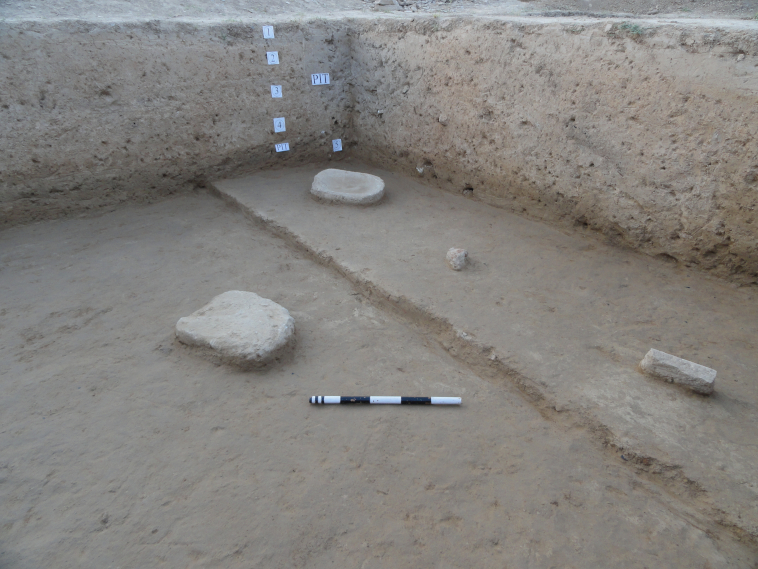
\includegraphics[scale=1.5]{images/chapter-3/fig006b.jpg}
\caption{LTS Pd. I Iron Age}\label{chapter-3-fig6B}
\end{figure}

\begin{figure}[H]
\renewcommand{\thefigure}{7A}
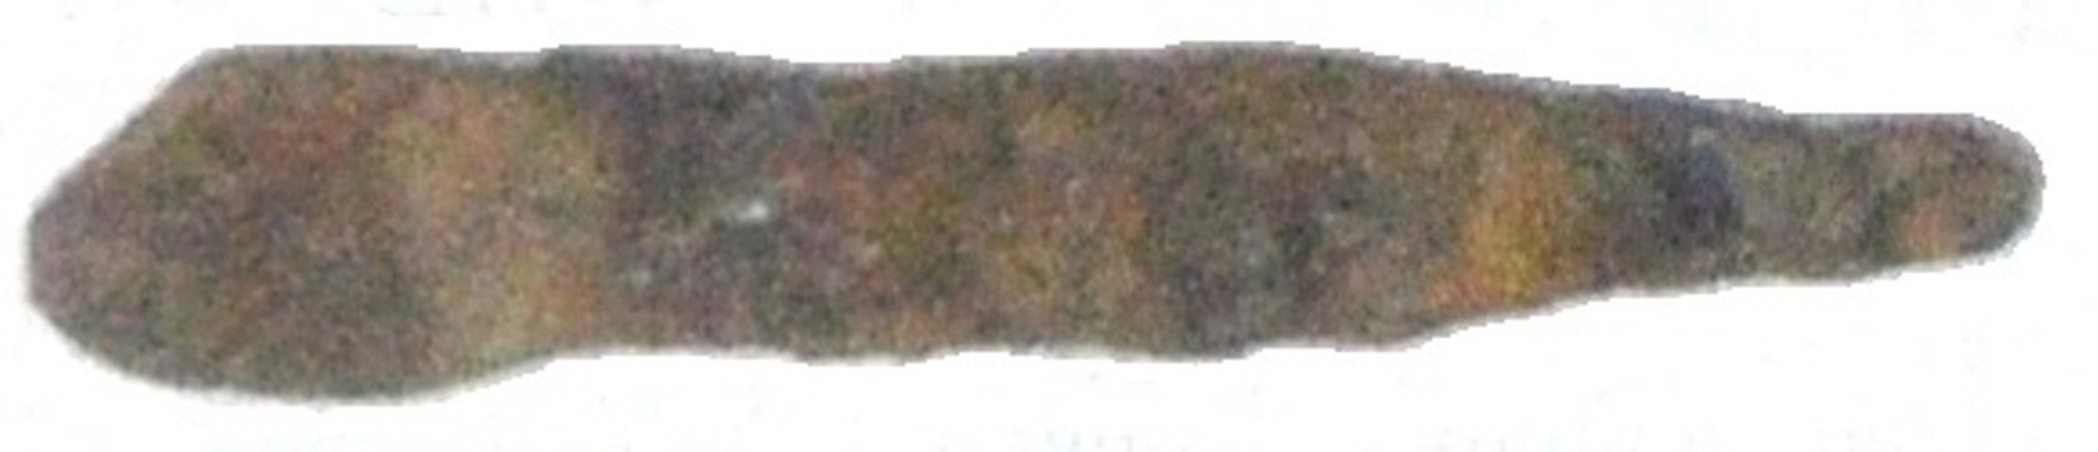
\includegraphics[scale=.5]{images/chapter-3/fig007a.jpg}
\caption{LTS 210 Surgical Knife Pd. III (1)}\label{chapter-3-fig7A}
\end{figure}

\begin{figure}[H]
\renewcommand{\thefigure}{7B}
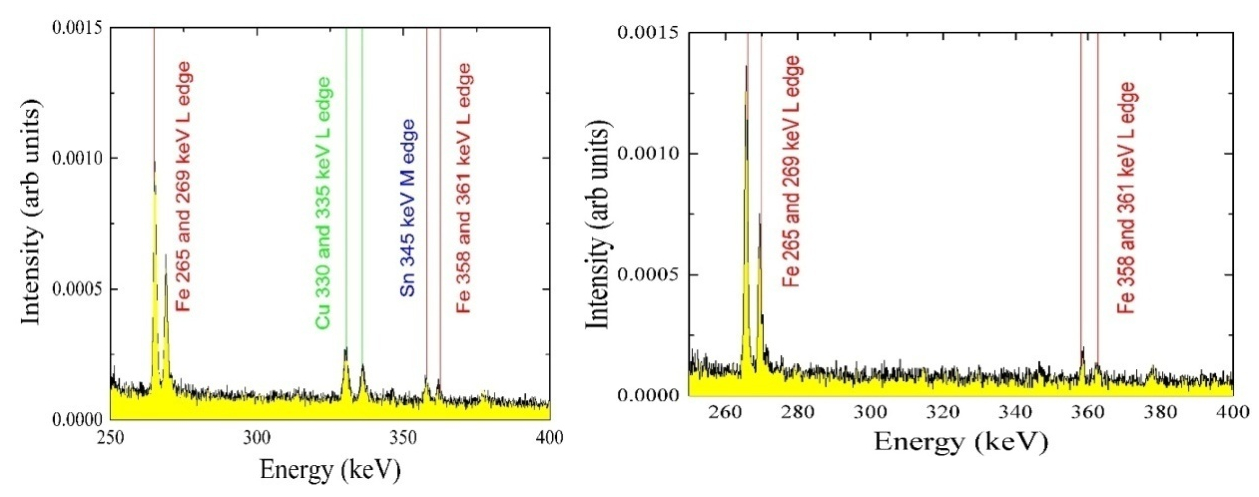
\includegraphics[scale=0.22]{images/chapter-3/fig007b.jpg}
\caption{LTS Pd. I Iron Age}\label{chapter-3-fig7B}
\end{figure}

Summarising the discussion, we may state that on the basis of the aforesaid, we can reconstruct and synthesise the disjointed evidence spanning over centuries. The evidence if culled down shows that there is a strong case of indigenous origin of iron in India. The radiocarbon dated number of them going back to 18/1700 BCE that too from sites in the heartland of India reiterate an independent origin of iron. We witness a process of beginning, development and survival of iron technology in the Vindhya-Kamur region as well as in southern India. We come across a pattern of innovations and technology adaptation. It also manifests the ingenuity displayed by the ironworkers of this region – a feature that continued to exist throughout the ages almost till the present. They could successfully meet the rising social demands with their innovative skill. The technological innovations led to material prosperity and socio-political reorganization and rise of cities in the Ganga Plain by $6^{\rm th}$ century BCE. 

{\setcounter{table}{0}
\renewcommand{\thetable}{III.\arabic{table}}
{\setlength\tabcolsep{2pt}
{\fontsize{7}{9}\selectfont
\begin{longtable}{|p{1.1cm}|c|p{1.4cm}|p{1cm}|p{.8cm}|p{.8cm}|p{1.1cm}|p{1.5cm}|}
\captionsetup{font=footnotesize}
\caption{Radiocarbon Dates of Jhusi}\label{table III.1}\\
\hline
\multicolumn{1}{|m{1.1cm}|}{\centering \textbf{Sl. No}}& & \multicolumn{1}{m{1.4cm}|}{\centering \textbf{Trench details}} & \multicolumn{3}{m{3cm}|}{\centering \textbf{Radiocarbon yrs BP}} & \multicolumn{1}{m{1.1cm}|}{\centering \textbf{Date in BCE/AD}} & \multicolumn{1}{m{1.5cm}|}{\centering \textbf{Calibrated dates in BCE/AD}}\\
& & &  \multicolumn{1}{c}{~~~~} & \multicolumn{1}{c}{5568$\pm$30} & \multicolumn{1}{c|}{5730$\pm$40} & & \\
\endfirsthead
\hline
\endhead
\hline
\endfoot
\hline
AU/JHS/1 & 2068 & C-12(12) 510 & Kushan & \hbox{1850$\pm$80} & \hbox{1910$\pm$90} & \hbox{40$\pm$90} AD & AD 74 (133) 316\\
AU/JHS/3 & 2070& C-14(30) 555 & Late NBP& 2104$\pm$90& 2200$\pm$90& 250$\pm$90 BCE& 357 (195, 173) 46 BCE\\
AU/JHS/6 & 2070 & C-15(37)1025 & Mid NBP& 2430$\pm$90& 2500$\pm$90& 550$\pm$90 BCE& 763 (498, 413) 393 BCE\\
AU/JHS/8 & 2074 & C-15 (43) 1165 & Early NBP & 2520$\pm$90 & 2590$\pm$90 & 640$\pm$90 BCE & 799 (763, 676, 674) 393 BCE\\
AU/JHS/9 & 2075 & C-15 (46) 1210 &  Pre~NBP with iron & 2650$\pm$90 & 2730$\pm$90 & 780$\pm$90 BCE & 897 (806) 789 BCE\\
AU/JHS/12 & 2077 & C-15 (49) 1240 & Pre NBP with iron  & 2820$\pm$90 & 2900$\pm$90 & 950$\pm$90 BCE & 1107 (973, 956, 941) 844 BCE\\
AU/JHS/16 & 2081 & C-15 (53) 1325 & Pre iron (Chalcolithic) & 2700$\pm$90 & 2780$\pm$90  & 830$\pm$90 BCE & 966 (830) 799 BCE\\
AU/JHS/18 & 2083 & C-15 (62) 1520  & Pre iron (Chalcolithic) & 3200$\pm$90 & 3290$\pm$90 &1340$\pm$90 BCE & 1597 (1490, 480, 1450) 1400 BCE\\
%\hline
\end{longtable}
}}

\vspace{-.5cm}

{\setlength\tabcolsep{2pt}
{\fontsize{7}{9}\selectfont
\begin{longtable}{|c|p{1.8cm}|p{1.5cm}|p{1.5cm}|p{1.5cm}|p{1.8cm}|}
\captionsetup{font=footnotesize}
\caption{Radiocarbon Dates of Raja Nal-Ka-Tila}\label{table III.2}\\
\hline
\multicolumn{1}{|m{.5cm}|}{\textbf{Sl. No}} &\multicolumn{1}{m{1.8cm}|}{\centering \textbf{Laboratory Number}}&\multicolumn{1}{m{1.5cm}|}{\centering \textbf{Layer/Depth}}&\multicolumn{1}{m{1.5cm}|}{\centering \textbf{Radiocarbon dates in years BP/BCE 5568$\pm$110 BP}}&\multicolumn{1}{m{1.5cm}|}{\centering \textbf{Calibrated dates based on half life 5530$\pm$40 years}} & \multicolumn{1}{m{1.8cm}|}{\centering \textbf{Calibrated}}\\
\endfirsthead
\hline
\endhead
\hline
\endfoot
\hline
1. & BS-1378 1996-97 Trench No. U-19 & (6) 1.95-2.00$\#$m With iron & 2550$\pm$110 BP 600$\pm$l10 BCE & 2626$\pm$110 BP 676$\pm$110 BCE & 822 (773) 486 BCE\\
2. & PRL-2047 1996-97 Trench No. U-20 & (6) 2.08-2.10$\#$m With iron & 2890$\pm$90 BP 940$\pm$90 BCE & 2980$\pm$90 BP 1030$\pm$90 BCE & 1196 BC-1188 BCE 1164 BC-1143 BCE 1132 BC-976 BCE 970 BC-930 BCE\\
3. & BS –1299 1995-96 Trench No. A-l & Pit sealed by layer No. (6) With iron & 2830$\pm$100 BP 880$\pm$100 BCE & 2914$\pm$100 BP 960$\pm$100 BCE & 1118 (963) 859 BCE\\
4. & BS –1300 1995-96 Trench No. A-l & (6) 2.00\#m With iron & 3060$\pm$110 BP 1110$\pm$110 BCE & 3150$\pm$110 BP 1200$\pm$110 BCE & 1423(1307) 1144 BCE\\
5. & PRL-2049 1996-97 Trench No. T-19 & (6) 2.00\#m With iron & 3050$\pm$90 BP 1100$\pm$90 BCE & 3150$\pm$90 BP 1200$\pm$90 BCE & 1406 BC -1198 BCE 1186 BC-1164 BCE 1143 BC-1132 BCE\\
6. & PRL - 2046 1996-97 Trench No. U-19 & (9) 2.80\#m Without iron & 3100$\pm$90 BP 1150$\pm$90 BCE & 3200$\pm$90 BP 1250$\pm$90 BCE & 1500 BC -1490 BCE 1448 BC-1256 BCE 1240 BC-1214 BCE\\
7. & PRL -2045 1996-97 Trench No. U-20 & (10) 2.90\#m Without iron & 3260$\pm$90 BP 1310$\pm$90 BCE & 3360$\pm$90 BP 1410$\pm$90 BCE & 1622 BC -1426 BCE 1742 BC-1378 BCE 1348 BC-1316 BCE\\
%\hline
\end{longtable}
}}


{\setlength\tabcolsep{2pt}
{\fontsize{7}{9}\selectfont
\begin{longtable}{|c|p{3.2cm}|p{1.5cm}|p{1.5cm}|p{1.8cm}|}
\captionsetup{font=footnotesize}
\caption{Radiocarbon Dates of Malhar}\label{table III.3}\\
\hline
\multicolumn{1}{|m{.5cm}|}{\centering \textbf{Sl. No}} &\multicolumn{1}{m{3.2cm}|}{\centering \textbf{Laboratory Number}}&\multicolumn{2}{m{3cm}|}{\centering \textbf{Radiocarbon dates in BP/BCE on the basis of half life 5568$\pm$30 years 5730$\pm$40 years}} &\multicolumn{1}{m{1.8cm}|}{\textbf{Cal BCE Stuiver {\it et.al.} one sigma}}\\
\hline
1. & BS - 1623, MLR II Trench No. XAl, Layer No. (3) Depth 0.55 cm & 3450$\pm$90 BP 1500$\pm$90 BCE & 3550$\pm$90 BP 1600$\pm$90 BCE & 1882 (1743) 1639 BCE\\
2. & BS - 1614, MLR II Trench No. Al, Layer No. (3) Depth 61-63cm & 6380$\pm$110 BP 4330$\pm$110 BCE & 6570$\pm$110 BP 4620$\pm$110 BCE & 5475 (5358, 5351, 5340, 5329, 5323) 5262 BCE\\
3. & BS - 1593, MLR II Trench No. Al, Layer No. (3) Depth 90-100cm &  3540$\pm$90 BP 1590$\pm$90 BCE & 3650$\pm$90 BP 1700$\pm$90 BCE & 2012 (1882,1836,34) 1742 BCE\\
4. & BS - 1590, MLR II Trench No. XAl, Layer No. (4) Depth 80cm & 3740$\pm$80 BP 1790$\pm$80 BCE & 3850$\pm$80 BP 1900$\pm$80 BCE & 2283 (2141) 1984 BCE\\
\hline
\end{longtable}
}}

{\setlength\tabcolsep{2pt}
{\fontsize{7}{9}\selectfont
\begin{longtable}{|c|p{1cm}|p{1.5cm}|p{1.5cm}|p{1.5cm}|p{1.3cm}|}
\captionsetup{font=footnotesize}
\caption{DATES OF BLACK-AND-RED WARE SITES\\[10pt]
(All BP dates are based on 5568 years half-life of Radiocarbon. \\
Calibrated dates are given in BCE/ AD. After Possehl 1994.)}\label{table III.4}\\
\hline
\multicolumn{1}{|m{1cm}|}{\centering \textbf{Site}} &\multicolumn{1}{m{1cm}|}{\centering \textbf{Sample No.}}&\multicolumn{1}{m{1.5cm}|}{\centering \textbf{5568 Yrs. BP}} &\multicolumn{1}{m{1.5cm}|}{\centering \textbf{Calibrated dates}} & \multicolumn{1}{m{1.5cm}|}{\centering \textbf{Culture}} & \multicolumn{1}{m{1.4cm}|}{\centering \textbf{Material}}\\
\endfirsthead
\hline
\endhead
\hline
\endfoot
\hline
Chirand & TF-336 & 2640$\pm$95 BP & 809 cal. BCE & Black-and-Red Ware Period Iron & Charcoal\\
Khairadih & PRL -1049 & 2890$\pm$150 BP & 484,437,424 cal. BCE & Black-and-Red Ware & Charcoal\\
Kilayur & TF-207 & 2200$\pm$100 BP & 353,306,236 cal. BCE & Black-and-Red Ware & Wood\\
Mahisdal & TF-389 & 2565$\pm$105 BP & 794 cal. BCE & Early Iron Age & Charcoal\\
Rajghat & TF-294 & 2190$\pm$85 BP & 348,316,207 cal. BCE & Black-and-Red Ware & Charcoal\\
Rajghat & TF-292 & 2350$\pm$95 BP & 400 cal. BCE & Black Slipped Ware & Charcoal\\
Sohgaura & PRL-178 & 3190$\pm$110BP & 1491,1489, 1451 cal. BCE & Black-and-Red Ware Chalcolithic & Charcoal\\
Sohgaura & PRL-179 & 3090$\pm$130 BP & 1400 cal. BCE & Black-and-Red Ware Chalcolithic & Charcoal\\
Sringaverpura & PRL-669 & 2620$\pm$130 BP & 805 cal. BCE & Black-and-Red Ware & Charcoal\\
Ujjain  & TF-407 & 1990$\pm$100 BP & 8 cal. AD & Black-and-Red Ware & Charcoal
\end{longtable}
}}

{\setlength\tabcolsep{2pt}
{\fontsize{7}{9}\selectfont
\begin{longtable}{|c|p{1.4cm}|p{1cm}|p{1.5cm}|p{3cm}|}
\captionsetup{font=footnotesize}
\caption{PGW SITES\\[10pt] 
All BP dates are based on 5568 yr half-life of Radiocarbon.\\ 
Calibrated dates are given in BCE/AD.}\label{table III.5}\\
\hline
\multicolumn{1}{|m{1cm}|}{\centering \textbf{Site}} &\multicolumn{1}{m{1.4cm}|}{\centering \textbf{Sample No.}}&\multicolumn{1}{m{1cm}|}{\centering \textbf{5568Yrs. BP}}& \multicolumn{1}{m{1.5cm}|}{\centering \textbf{Calibrated dates}}& \multicolumn{1}{m{3cm}|}{\centering \textbf{Culture}}\\
\endfirsthead
\hline
\endhead
\hline
\endfoot
\hline
Hastinapur & TF-90 & 2270$\pm$110 & 383 cal. BCE & Upper-most painted Grey ware, Period II, \\
Hastinapur & TF-112 & 2260$\pm$95 & 379 cal. BCE & Upper most Painted Grey ware, period II\\
Hastinapur & UCLA-684 &1800$\pm$100 & 227 cal. AD & Painted Grey ware Period II, Probably an intrusive burial?\\
Hastinapur & TF-85 & 2385$\pm$l25 & 406 cal. BCE & Late Painted Grey ware, Period II\\
Hastinapur & TF-83 & 2220$\pm$ll0 & 362,282,258 cal. BCE & Uppermost Painted Grey ware, Period II\\
Hastinapur & TF-91 & 2450$\pm$l20 & 752,709,530 cal. BCE & Late Painted Grey ware, Period II\\
Hulas & PRL-HLS-TL-l & None & None &  Period II, Painted Grey ware, late phase\\
Khalaua & PRL-67 & 2450$\pm$155 & 752,709.530 ca1. BCE & Painted Grey ware\\
Khalaua & TF-1228 & 2420$\pm$95 & 484.437.424 ca1. BCE & Painted Grey ware\\
Khalaua & PRL-68 & 2370$\pm$170 & 403 ca1. BCE & Painted Grey ware\\
Noh & TF-1144 & 2370$\pm$85 & 403 ca1. BCE & Painted Grey ware\\
Noh & TF -994 & 2560$\pm$100 & 794 BCE & Painted Grey ware\\
Noh & UCLA- 703A & 2480$\pm$250 & 760.684.656 638.592.586 550 ca1. BCE & Painted Grey ware\\
Noh & UCLA-703B & 2690$\pm$220 & 833 ca1. BCE &Painted Grey ware\\
Noh & TF-993 & 2600$\pm$145 & 801 cal. BCE &Painted Grey ware\\
Sonkh & 1-6277 & 2570$\pm$85 & 795 cal. BCE &Painted Grey ware\\
Mound & & & & \\
Mathura & & & & \\
Sonpur & TF-376 & 2510$\pm$105 & 767 cal. BCE &Pre-NBP\\
Thapli & PRL- 732 & 2070$\pm$120 & 101 cal. BCE & PGW\\
Thapli & PRL- 731 & 2030$\pm$140 & 43 cal. BCE &PGW\\
Tilaurakot & TF-737 & 2235$\pm$95 & 368,273,268 cal. BCE &PGW\\
Jodhpura & PRL-212 & 2270$\pm$100 & 383 cal. BCE Painted Grey ware overlap & Black \& Red ware
\end{longtable}
}}

{\setlength\tabcolsep{2pt}
{\fontsize{8}{10}\selectfont
\begin{longtable}{|c|p{1.1cm}|p{1.2cm}|p{1.8cm}|p{3.3cm}|}
\captionsetup{font=footnotesize}
\caption{Radiocarbon and TL Dates of NBP Ware and Early Iron Sites\\
(India and Pakistan)\\ [5pt]
All BP dates are based on 5568 yr half-life of Radiocarbon. \\[3pt] 
Calibrated dates are given in BCE/AD.\label{table III.6}}\\
\hline
\multicolumn{1}{|m{1.3cm}|}{\centering \textbf{Site}} &\multicolumn{1}{m{1.1cm}|}{\centering \textbf{Sample No.}}&\multicolumn{1}{m{1.2cm}|}{\centering \textbf{Date BP/5568 yr half life}}& \multicolumn{1}{m{1.8cm}|}{\centering \textbf{Calibrated dates}}& \multicolumn{1}{m{3.3cm}|}{\centering \textbf{Culture/level}}\\
\endfirsthead
\multicolumn{5}{r}{\textbf{(\textit{continued})}}\\[5pt]
\hline
\multicolumn{1}{|m{1.3cm}|}{\centering \textbf{Site}} &\multicolumn{1}{m{1.1cm}|}{\centering \textbf{Sample No.}}&\multicolumn{1}{m{1.2cm}|}{\centering \textbf{Date BP/5568 yr half life}}& \multicolumn{1}{m{1.8cm}|}{\centering \textbf{Calibrated dates}}& \multicolumn{1}{m{3.3cm}|}{\centering \textbf{Culture/level}}\\
\hline
\endhead
\hline
\multicolumn{5}{r}{\small\itshape continued on the next page}\\
\endfoot
\endlastfoot
\hline
Atranjikhera & TF-283 & 2150$\pm$105 & 192 cal. BCE &Northern Black Polished Ware, Period IV\\
Atranjikhera & BM-193 & 2040$\pm$150 & 50 cal. BCE & Painted Grey Ware/ Northern Black Polished Ware overlap\\
Atranjikhera & TF-415 & 2450$\pm$200 & 752,709,530 \hbox{cal. BCE} & Period II, Black and Red ware\\
Atranjikhera & TF-289 &2550$\pm$105 &791 cal. BCE &Period II, Black and Red ware\\
Atranjikhera & TF-194 & 2410$\pm$85 &410 cal. BCE &Painted Grey Ware, Period III\\
Atranjikhera & TF-291 &2415$\pm$100 & 512 cal. BCE &Painted Grey Ware, Period III\\
& BM-194 & 2420$\pm$150 & 484,437,424 \hbox{cal. BCE} & Painted Grey Ware/ Northern Black Polished Ware overlap\\
Atranjikhera & TF-191 & 2890$\pm$105 & 1057 cal. BCE & Painted Grey Ware, Period III\\
Atranjikhera & TF-287 & 1605$\pm$95 & 427 cal. AD &Painted Grey Ware, Period III\\
Atranjikhera & TF-284 & 2180$\pm$95 & 340,322.203 \hbox{cal. BCE} & Northern Black Polished Ware, Period IV\\
Atranjikhera & TF-195 & 1845$\pm$95 & 137 cal. AD & Post-Northern Black Polished ware, Period IV\\
Atranjikhera & UW-XXXX & 2407$\pm$150 & 489 cal. BCE & Painted Grey Ware/Northern Black Polished Ware overlap\\
Atranjikhera & OXFORD- TL-ll1-C1 & 2280 & None & Ochre Coloured Pottery. Period I\\
Atranjikhera & OXFORD- TL-ll1-B4 & 1670 & None & Ochre Coloured Pottery. Period I\\
Atranjikhera & OXFORD- TL-ll1-B5 & 1170 & None & Ochre Coloured Pottery. Period I\\
Atranjikhera & OXFORD- TL-ll1-C2 & 1250 & None & Ochre Coloured Pottery, period I\\
Atranjikhera & OXFORD- TL-111-C3 & 2130 & None & Ochre Coloured Pottery. Period I\\
Hastinapur & TF-88 & 2225$\pm$110 & 340$\pm$115 BCE, 364, 279, 261 cal. BCE &\\
Hastinapur & TF-80/82 & 1940$\pm$110 & 50$\pm$115 BCE, 66 AD &\\
Hastinapur & TF-81 & 2015$\pm$95 & 125$\pm$100 BCE, 32 cal. BCE &\\
Hetimpur & TF-176 & 2000$\pm$100 & 110$\pm$105 BCE, 1cal. BCE &\\
Hetimpur & TF-l77 & 1820$\pm$100 & 75$\pm$105 AD, 214 cal. AD &\\
Kausambi & TF-225 & 2285$\pm$105 & 405$\pm$l10 BCE, 390 cal. BCE &\\
Kausambi & TF-I05 & 2220$\pm$llO & 335$\pm$115 BCE, 362, 282, 258 cal. BC & \\
Kausambi & TF-I03 & 2295$\pm$l05 & 415$\pm$ll0 BC, 391 cal. BCE &\\
Kausambi & TF-219 & 2325$\pm$l00 & 445$\pm$l05 BCE, 396 cal. BCE &\\
Kausambi & TF-221 & 2385$\pm$l00 & 505$\pm$105 BCE, 406 cal. BCE &\\
Kausambi & TF-226 & 2110$\pm$95 & 225$\pm$l00 BCE, 160, 138, 124 cal. BCE &\\
Kausambi & TF -100 & 2160$\pm$95 & 275$\pm$100 BCE, 196 cal. BCE & \\
Kausambi & TF-I04 & 2150$\pm$105 & 265$\pm$100 BCE, 192 cal. BCE &\\
Kayatha & TF-674 & 2350$\pm$95 & 470$\pm$l00 BCE, 400 cal. BCE &\\
Kayatha & TF-394 & 2380$\pm$95 & 500$\pm$100 BCE, 405 cal. BCE & \\
Khairadih & PRL-I050 & 2060$\pm$150 & 170$\pm$150 BCE, 96 cal. BCE & \\
Manjhi & PRL-980 & 1930$\pm$140 & 37$\pm$145 BCE, 72 cal. AD &\\
Manjhi & PRL-983 & 2350$\pm$140 & 470$\pm$145 BCE, 400 cal. BCE & \\
Mathura & PRL-343 & 2150$\pm$100 & 265$\pm$l05 BCE, 192 cal. BCE &\\
Mathura & PRL-340 & 2390$\pm$150 & 510$\pm$155 BCE, 407 cal. BCE& \\
Mathura & PRL-333 & 2490$\pm$140 & 615$\pm$145 BCE, 762, 678, 662, 627, 600 cal. BCE &\\
Mathura & PRL-338 & 2280$\pm$100 & 400$\pm$105 BCE, 387 cal. BCE &\\
Mathura & PRL-342 & 2180$\pm$160 & 295$\pm$165 BCE, 340, 322, 203 cal. BCE & \\
Mathura & PRL-339 & 2380$\pm$100 & 500$\pm$105 BCE, 405 cal. BCE &\\
Mathura & PRL-337 & 2340$\pm$100 & 460$\pm$105 BCE, 399 cal. BCE &\\
Mathura & PRL-336 & 2540$\pm$90 & 665$\pm$95 BCE, 786 cal. BCE &\\
Mathura & PRL-334 & 2600$\pm$150 & 730$\pm$155 BCE, 801 cal. BCE & \\
Narhan & BS-563 & 2240$\pm$100 & 355$\pm$105 BCE, 370 cal. BCE & \\
Narhan & BS-564 & 2200$\pm$100 & 315$\pm$105 BCE, 353, 306, 236 cal. BCE & \\
Narhan & BS-581 & 2100$\pm$100 & 215$\pm$105 BCE, 151, 149, 117 cal. BCE & \\
Rajghat & TF -293 & 2370$\pm$105 & 490$\pm$1l0 BCE, 403 cal. BCE & \\
Ropar & TF-209 & 2365$\pm$100 & 485$\pm$105 BCE, 403 cal. BCE & \\
Ropar & TF-213 & 2275$\pm$100 & 395$\pm$105 BCE, 385 cal. BCE & \\
Semthan & PRL-946 & 1880$\pm$120 &15$\pm$125AD, 118 cal. BCE &\\
Semthan & PRL-945 & 2280$\pm$110 & 400$\pm$115 BCE, 387cal. BCE & \\
Semthan & PRL-941 & 2200$\pm$140 & 315$\pm$145 BCE, 353, 306, 236 cal. BCE &\\
Sohgaura & PRL-182A & 2130$\pm$90 & 245$\pm$95 BCE, 177 cal. BCE & \\
Sohgaura & PRL-183 & 2466$\pm$105 & 590$\pm$110 BCE, 756, 692, 541 cal. BCE &\\
Sohgaura & PRL-182B & 2290$\pm$400 & 410$\pm$410 BCE, 391cal. BCE &\\
Pirak & LY-1643 &n 2970$\pm$140 & 1110$\pm$145 BCE, 1255, 1240, 1221 cal. BCE&\\
\hline
\end{longtable}
}}

{\setlength\tabcolsep{2pt}
{\fontsize{7}{9}\selectfont
\begin{longtable}{|p{1.5cm}|p{1cm}|p{1.2cm}|p{1.8cm}|p{2.5cm}|}
\captionsetup{font=footnotesize}
\caption{South Indian Megaliths\\
All BP dates are based on 5568 yr half-life of Radiocarbon. \\
Calibrated dates are given in BCE/AD.}\label{table III.7}\\
\hline
\multicolumn{1}{|m{1.5cm}|}{\centering \textbf{Site}} &\multicolumn{1}{m{1cm}|}{\centering \textbf{Sample No.}}&\multicolumn{1}{m{1.2cm}|}{\centering \textbf{Date BP/5568}} & \multicolumn{1}{m{1.8cm}|}{\centering \textbf{Calibrated dates}}& \multicolumn{1}{m{2.5cm}|}{\centering \textbf{Culture}}\\
\endfirsthead
\hline
\endhead
\hline
\endfoot
\hline
Halingali & TF-685 & 1970$\pm$95 & 22 cal. AD & Megalithic Neolithic\\
Hallur & TF-570 & 2970$\pm$105 & 1255,1240,221 cal. BCE & Period II, Neolithic/ Iron Age Overlap\\
Hallur & TF -573 & 2820$\pm$l00 & 993 cal. BCE & Period II, Neolithic/ Iron Age Overlap\\
Hathinia Hill & TF-I09 & 30$\pm$90 & 1955 cal. AD & Megalithic\\
Korkai & TF-987 & 2680$\pm$90 & 828 cal. BCE & Megalithic, Ancient port\\
Naikund & BS-94 & 2495$\pm$105 & 763,675,665, 620, 604 cal. BCE &Megalithic\\
Naikund & BS-92 & 2455$\pm$100 & 753,704,533 cal. BCE &Megalithic\\
Komaranhalli, Karnataka \hbox{(TL dates)}  & PRL-46 PRL-47 PRL-49 PRL-50 &&1320 400 1380 300 1130 500 1140 290 & \\
Veerampura, Andhra Pradesh & PRL-728 PRL-730 && 920 140 1200 140 & \\
Vidarbha, \hbox{Mahararastra} & PRL-1361  PRL-1452  PRL-1456 & 2940$\pm$160 3080$\pm$120 2820$\pm$100 & 1393 (1205, 1205, 1188, 1181, 1149, 1144, 1129) 917 1490 (1381, 1334, 1321) 1133 1185 (973, 956, 941) 834 & Unpublished information from the excavator
\end{longtable}
}}

{\setlength\tabcolsep{2pt}
{\fontsize{8}{10}\selectfont
\begin{longtable}{|c|p{1.6cm}|p{2cm}|p{2cm}|p{2cm}|}
\captionsetup{font=footnotesize}
\caption{${\rm C}^{14}$ dates for early iron bearing sites from the\\ Ganga Plain and the Eastern Vindhyas} \label{table III.8}\\
\hline
\multicolumn{1}{|m{.5cm}|}{\centering \textbf{Sl. No.}} &
\multicolumn{1}{m{1.6cm}|}{\centering \textbf{Laboratory Number}} &
\multicolumn{1}{m{2cm}|}{\centering \textbf{Radiocarbon dates in years BP/BCE 5568$\pm$110 BP}} & 
\multicolumn{1}{m{2cm}|}{\centering \textbf{Calibrated dates based on half life 5530$\pm$40 years}} & 
\multicolumn{1}{m{2cm}|}{\centering \textbf{Calibrated}}\\
\endfirsthead
\hline
\endhead
\hline
\endfoot
\hline
1. & BS-1378  & 2550$\pm$110 \hbox{BP 600$\pm$l10 BCE} & 2626$\pm$110 \hbox{BP 676$\pm$110 BCE} & 822 (773) 486 BCE\\
2. & PRL-2047  & 2890$\pm$90 \hbox{BP 940$\pm$90 BCE} & 2980$\pm$90 \hbox{BP 1030$\pm$90 BCE} & 1196 BC-1188 BCE 1164 BC-1143 BCE 1132 BC-976 BCE 970 BC-930 BCE \\
3. & BS –1299  & 2830$\pm$100 \hbox{BP 880$\pm$100 BCE} & 2914$\pm$100 \hbox{BP 960$\pm$100 BCE} & 1118 (963) 859 BCE\\
4. & BS –1300  & 3060$\pm$110 \hbox{BP 1110$\pm$110 BCE} & 3150$\pm$110 \hbox{BP 1200$\pm$110 BCE} & 1423(1307) 1144 BCE\\
5. & PRL-2049  & 3050$\pm$90 \hbox{BP 1100$\pm$90 BCE} & 3150$\pm$90 \hbox{BP 1200$\pm$90 BCE} & 1406 BC -1198 BCE 1186 BC-1164 BCE 1143 BC-1132 BCE\\
6. & PRL - 2046 1996-97 Trench No. U-19 & 3100$\pm$90 \hbox{BP 1150$\pm$90 BCE} & 3200$\pm$90 \hbox{BP 1250$\pm$90 BCE} &1500 BC -1490 BCE 1448 BC-1256 BCE 1240 BC-1214 BCE\\
7. & PRL -2045  & 3260$\pm$90 \hbox{BP 1310$\pm$90 BCE} & 3360$\pm$90 \hbox{BP 1410$\pm$90 BCE} & 1622 BC -1426 BCE 1742 BC-1378 BCE 1348 BC-1316 BCE
%\hline
\end{longtable}
}}

{\setlength\tabcolsep{2pt}
{\fontsize{7}{9}\selectfont
\begin{longtable}{|p{1.8cm}|p{2.5cm}|p{2cm}|p{2.5cm}|}
\captionsetup{font=footnotesize}
\caption{Radiocarbon Dates of Raipura (BSIP, Lucknow)} \label{table III.9}\\
\hline
\multicolumn{1}{|m{1.8cm}|}{\centering \textbf{Laboratory Number}} &
\multicolumn{1}{m{2.5cm}|}{\centering \textbf{Layer/ Depth}} & 
\multicolumn{1}{m{2cm}|}{\centering \textbf{Calibrated Age with 1 sigma}} & 
\multicolumn{1}{m{2.5cm}|}{\centering \textbf{Calibrated Age with 2 sigma}}\\
\endfirsthead
\hline
\endhead
\hline
\endfoot
\hline
BS\#3384 Charcoal Less Carbon\footnotemark & Tr. YI-11, Depth 60 cm, Floor 1 of Lr. (2) NBPW & 340 Cal BCE ($\pm$ 50) with 1 sigma & 400 Cal BCE ($\pm$ 200) with 2 sigma\\
BS\#3386 Charcoal &  Tr. YH-11, Depth 130- 135 cm, Pit 3 sealed by Lr. (2) NBPW & 430 Cal BCE ($\pm$ 80)  with 1 sigma & 460 Cal BCE ($\pm$ 100) with 2 sigma \\
BS\#3536 Charcoal & Tr. YI-11 90 cm, Pit sealed by Lr. (4) With Iron & 1720$\pm$220 cal BC with 1 sigma & \\
BS\#3545 Charcoal & Tr. YH-11, Depth 85 cm, Pit sealed by Lr. (3) Without iron & 2410$\pm$140 cal BC with 1 sigma & \\
BS\#3544 Charcoal &  Tr. YH-11, Depth 100-105 cm, Pit sealed by Lr. (4) Without iron & 2510$\pm$180 Cal. BC with 1 sigma & \\
BS\# 3387 Charcoal & Tr. ZB-10, Depth 140-145 cm, Pit 4 sealed by Lr.(5) Without iron & 2720 Cal BCE ($\pm$ 80)  with 1 sigma & 2690 Cal BCE ($\pm$ 230) with 2 sigma\\
BS\# 3385 Charcoal  & Tr. ZB-10, Depth 170-175 cm, Pit 5 sealed by Lr.(5) Without iron & 2770 Cal BCE ($\pm$ 80) with 1 sigma & 2790 Cal BCE ($\pm$ 310) with 2 sigma\\
BS\#3542 Charcoal & Tr. ZH-10, Depth 195-200cm, Pit sealed by Lr. (7) Without Iron & 2790$\pm$60 Cal. BC with 1 sigma & \\
BS\#3383 charcoal & Tr. ZH-10, Depth 170- 175 cm, Pit 7 sealed by Lr. (8) Without iron & 3270 Cal BCE ($\pm$ 130 ) with 1 sigma & 3240 Cal BCE ($\pm$ 290) with 2 sigma
\end{longtable}
\footnotetext{For the Sample No. BS\#3384, small amount of carbon implied loss of precision.}
}}

{\setlength\tabcolsep{2pt}
{\fontsize{7}{9}\selectfont
\begin{longtable}{|p{1.3cm}|p{1.6cm}|p{1.6cm}|p{4.4cm}|}
\captionsetup{font=footnotesize}
\caption{Radiocarbon Dates of Raipura (PRL Ahmadabad)} \label{table III.10}\\
\hline
\multicolumn{1}{|m{1.3cm}|}{\centering \textbf{Laboratory Number}} &
\multicolumn{1}{m{1.6cm}|}{\centering \textbf{Location of Sample}} & 
\multicolumn{1}{m{1.6cm}|}{\centering \textbf{C14- Age in yr BP (based on $\tau1/2=5730$ yr) }} & 
\multicolumn{1}{m{4.4cm}|}{\centering \textbf{Cal  BC with 1 sigma/ 2 sigma}}\\
\endfirsthead
\hline
\endhead
\hline
\endfoot
\hline
PRL-3317 BHU/RPA/1 & ZB-10, 145-150 cm, Pit SB Lr.(4)\par  With Iron Earliest level of Pd. II & 3480 ± 110 & One Sigma Ranges: [start:end] relative area \par [cal BC 1867: cal BC 1848] 0.055721 \par [cal BC 1774: cal BC 1527] 0.944279\par  Two Sigma Ranges: [start:end] relative area\par [cal BC 1932: cal BC 1438] 1.\\
PRL-3318 BHU/RPA/2  &  XJ-5, 165-170 cm, Pit SB Lr.(1) \par With Iron middle level of Pd. II & 2950 ± 140 & One Sigma Ranges: [start:end] relative area \par  [cal BC 1257: cal BC 1234] 0.054564 \par  [cal BC 1216: cal BC 899] 0.945436 \par  Two Sigma Ranges: [start:end] relative area \par  [cal BC 1395: cal BC 803] 1.\\
PRL-3320  BHU/RPA/4 & YI-11, 75-80 cm, Lr.(3)\par With Iron middle level of Pd. II & 3000 ± 80  & One Sigma Ranges: [start:end] relative area\par  [cal BC 1257: cal BC 1235] 0.077994 \par [cal BC 1216: cal BC 1006] 0.922006\par Two Sigma Ranges: [start:end] relative area \par [cal BC 1372: cal BC 1343] 0.022781 \par  [cal BC 1318: cal BC 911] 0.977219\\
PRL-3321 BHU/RPA/5  & YH-11, 125-130 cm, Pit SB Lr.(3) \par With Iron From upper layer of Pd. II & 2800 ± 90 & One Sigma Ranges: [start:end] relative area \par [cal BC 974: cal BC 957] 0.079577 \par [cal BC 940: cal BC 801] 0.920423 \par Two Sigma Ranges: [start:end] relative area \par  [cal BC 1128: cal BC 754] 0.990223 \par [cal BC 685: cal BC 668] 0.006721\par [cal BC 609: cal BC 598] 0.003057\\
PRL-3319 BHU/RPA/3  & YI-11, 60 cm,  Pit SB Floor 1, Lr.(2) \par With Iron Transitional phase of of Pd. II and Pd. III & 2680 ± 100  & One Sigma Ranges: [start:end] relative area \par  [cal BC 894: cal BC 873] 0.059897\par  [cal BC 849: cal BC 734] 0.497125\par  [cal BC 690: cal BC 662] 0.107593 \par  [cal BC 649: cal BC 546] 0.335386\par Two Sigma Ranges: [start:end] relative area\par  [cal BC 926: cal BC 413] 1.\\
PRL-3322  BHU/RPA/6 & YH-11, 25-30 cm, Lr.(1)\par With Iron From upper layer of Pd. III & 2260 ± 110 & One Sigma Ranges: [start:end] relative area \par [cal BC 387: cal BC 159] 0.939516 \par [cal BC 134: cal BC 116] 0.060484 \par Two Sigma Ranges: [start:end] relative area \par [cal BC 507: cal BC 459] 0.01665 \par [cal BC 453: cal BC 439] 0.004657 \par [cal BC 419: cal AD 31] 0.973106 \par [cal AD 37: cal AD 52] 0.005587
\end{longtable}
}}}

\theendnotes 

\label{endchapter3}
